% =============================================================================
%  IIIT RAICHUR -- B.Tech PROJECT THESIS TEMPLATE
%  Department of Computer Science and Engineering
%  -----------------------------------------------------------------------------
%  HOW TO USE
%   1. Edit the placeholder commands in the "USER INPUTS" block below.
%   2. Place your college logo at: images/iiitr_logo.png
%   3. Replace the lorem ipsum / dummy text with your own project content.
%   4. Add your figures to the images/ folder.
%   5. Compile:
%        pdflatex thesis.tex
%        pdflatex thesis.tex
%      (or simply: latexmk -pdf thesis.tex)
%
%  This template is domain-agnostic. The dummy text is generic so it works for
%  any kind of project -- software, hardware, embedded, ML, networking, etc.
% =============================================================================

\documentclass[12pt, a4paper, oneside]{report}

% ---------------------- PACKAGES ---------------------------------------------
\usepackage[utf8]{inputenc}
\usepackage[T1]{fontenc}
\usepackage{lmodern}
\usepackage[margin=1in, top=1.2in, bottom=1.2in]{geometry}
\usepackage{graphicx}
\usepackage{setspace}
\usepackage{titlesec}
\usepackage{tocloft}
\usepackage{fancyhdr}
\usepackage{booktabs}
\usepackage{longtable}
\usepackage{array}
\usepackage{tabularx}
\usepackage{multirow}
\usepackage{caption}
\usepackage{subcaption}
\usepackage{amsmath, amssymb}
\usepackage{xcolor}
\usepackage[hidelinks, breaklinks=true]{hyperref}
\usepackage{url}
\usepackage{enumitem}
\usepackage{float}
\usepackage{lipsum}    % provides \lipsum for lorem ipsum dummy text
\usepackage{listings}  % numbered pseudocode blocks

% ---- pseudocode listing style (line-numbered, framed) -----------------------
\lstdefinestyle{pseudo}{%
  basicstyle=\ttfamily\footnotesize,
  numbers=left,
  numberstyle=\scriptsize\color{gray},
  numbersep=10pt,
  stepnumber=1,
  frame=single,
  rulecolor=\color{gray!45},
  framesep=4pt,
  xleftmargin=24pt,
  framexleftmargin=18pt,
  aboveskip=0.4em,
  belowskip=1.0em,
  columns=fullflexible,
  keepspaces=true,
  breaklines=true,
  breakatwhitespace=true,
  showstringspaces=false,
  tabsize=2,
}
% bold heading printed immediately above a pseudocode block
\newcommand{\algname}[1]{\par\vspace{0.6em}\noindent\textbf{\ttfamily #1}\nopagebreak}

% ---------------------- USER INPUTS (EDIT THESE) -----------------------------
% Plain title (single line) -- used in declaration, certificate, abstract.
\newcommand{\thesisTitle}{FinITR-AI: An Agentic Multi-Document Reconciliation System for Indian Income Tax Return Filing}
% Display title (with line breaks) -- used only on the title page.
% Add \\ wherever you want a line break for visual layout.
\newcommand{\thesisTitleDisplay}{FinITR-AI \\ AN AGENTIC MULTI-DOCUMENT RECONCILIATION SYSTEM \\ FOR INDIAN INCOME TAX RETURN FILING}
\newcommand{\studentName}{<< YOUR FULL NAME >>}
\newcommand{\rollNumber}{<< YOUR ROLL NO >>}
\newcommand{\supervisorName}{Dr.~<< SUPERVISOR NAME >>}
\newcommand{\departmentName}{Computer Science and Engineering}
\newcommand{\submissionMonthYear}{May 2026}
\newcommand{\submissionLocation}{Raichur -- 584135}
\newcommand{\degreeName}{Bachelor of Technology}
\newcommand{\logoPath}{images/iiitr_logo.png}

% ---------------------- FORMATTING -------------------------------------------
\onehalfspacing

% Chapter title formatting (matches "Chapter N" on top, title below)
\titleformat{\chapter}[display]
  {\normalfont\huge\bfseries}{\chaptertitlename\ \thechapter}{20pt}{\Huge}
\titlespacing*{\chapter}{0pt}{-30pt}{30pt}

% Page style -- page number at bottom centre, no header rule
\pagestyle{fancy}
\fancyhf{}
\fancyfoot[C]{\thepage}
\renewcommand{\headrulewidth}{0pt}
\renewcommand{\footrulewidth}{0pt}

\fancypagestyle{plain}{%
  \fancyhf{}%
  \fancyfoot[C]{\thepage}%
  \renewcommand{\headrulewidth}{0pt}%
  \renewcommand{\footrulewidth}{0pt}%
}

% TOC formatting
\renewcommand{\cftchapfont}{\bfseries}
\renewcommand{\cftchappagefont}{\bfseries}

% Helper command for centered front-matter headings (Declaration, Certificate, Abstract)
\newcommand{\frontmatterheading}[1]{%
  \begin{center}\Large\bfseries #1\end{center}
  \vspace{0.5cm}
}

% Paragraph spacing
\setlength{\parskip}{0.5em}
\setlength{\parindent}{1.5em}

% =============================================================================
\begin{document}

% ---------------------- TITLE PAGE -------------------------------------------
\begin{titlepage}
    \centering
    \thispagestyle{empty}
    \vspace*{0.2cm}

    {\Large\bfseries \thesisTitleDisplay \par}
    \vspace{0.8cm}

    {\normalsize A Project Report Submitted \par}
    {\normalsize in Partial Fulfilment of the Requirements \par}
    {\normalsize for the Degree of \par}
    \vspace{0.5cm}

    {\large\bfseries \MakeUppercase{\degreeName} \par}
    \vspace{0.3cm}

    {\normalsize in \par}
    \vspace{0.2cm}

    {\large\bfseries \MakeUppercase{\departmentName} \par}
    \vspace{0.5cm}

    {\normalsize\itshape by \par}
    \vspace{0.3cm}

    {\normalsize\bfseries \studentName{} (Roll No.~\rollNumber) \par}
    \vspace{0.5cm}

    % College logo
    \includegraphics[width=1\textwidth]{\logoPath}\par
    \vspace{0.5cm}

    {\normalsize\itshape to \par}
    \vspace{0.2cm}

    {\normalsize\bfseries DEPARTMENT OF \MakeUppercase{\departmentName} \par}
    {\normalsize\bfseries INDIAN INSTITUTE OF INFORMATION TECHNOLOGY \par}
    {\normalsize\bfseries RAICHUR-584135, INDIA \par}
    \vspace{0.4cm}

    {\normalsize\itshape \submissionMonthYear \par}

\end{titlepage}

% ---------------------- FRONT MATTER (roman page numbers) --------------------
\pagenumbering{roman}
\setcounter{page}{2}

% ---------------------- DECLARATION ------------------------------------------
\clearpage
\thispagestyle{plain}
\frontmatterheading{DECLARATION}
\addcontentsline{toc}{chapter}{Declaration}

\noindent I \textbf{\MakeUppercase{\studentName}} (Roll Number: \rollNumber) hereby
declare that, this report entitled ``\textit{\thesisTitle}'' submitted to
Indian Institute of Information Technology Raichur towards partial requirement
of \degreeName{} in \departmentName{} is an original work carried out by me
under the supervision of Mentor, \supervisorName{} and has not formed the
basis for the award of any degree or diploma, in this or any other institution
or university. I have sincerely tried to uphold the academic ethics and
honesty. Whenever an external information or statement or result is used then,
that have been duly acknowledged and cited.

\vspace{2.5cm}
\noindent
\begin{minipage}[t]{0.5\textwidth}
\submissionLocation \\
\submissionMonthYear
\end{minipage}
\hfill
\begin{minipage}[t]{0.4\textwidth}
\raggedleft
\studentName \\
Roll No.~\rollNumber
\end{minipage}

% ---------------------- CERTIFICATE ------------------------------------------
\clearpage
\thispagestyle{plain}
\frontmatterheading{CERTIFICATE}
\addcontentsline{toc}{chapter}{Certificate}

\noindent This is to certify that the work contained in this project report
entitled ``\textit{\thesisTitle}'' submitted by \textbf{\studentName} (Roll
No: \rollNumber) to the Indian Institute of Information Technology Raichur
towards partial requirement of \degreeName{} in \departmentName{} has been
carried out by him/her under my supervision and that it has not been submitted
elsewhere for the award of any degree.

\vspace{3cm}
\noindent
\begin{minipage}[t]{0.5\textwidth}
\submissionLocation \\
\submissionMonthYear
\end{minipage}
\hfill
\begin{minipage}[t]{0.4\textwidth}
\raggedleft
(\supervisorName) \\
Project Supervisor
\end{minipage}

% ---------------------- ABSTRACT ---------------------------------------------
\clearpage
\thispagestyle{plain}
\frontmatterheading{ABSTRACT}
\addcontentsline{toc}{chapter}{Abstract}

% ---- ABSTRACT CONTENT ----
% ============================================================================
%  ABSTRACT  ->  replaces \lipsum[1] and \lipsum[2][1-5] under the
%  \frontmatterheading{ABSTRACT} block in main.tex (~line 213)
% ============================================================================

Every year, millions of salaried Indians file their income tax returns while
sitting on an awkward information gap: the Income Tax Department already knows
about most of their financial activity through the Annual Information Statement
(AIS), yet the tools people use to file still work almost entirely from
self-reported numbers. When the two views disagree, the taxpayer is the last to
find out -- usually through a Section 143(1) notice months later. This thesis
presents FinITR-AI, a locally-runnable, multi-agent system that closes that gap
by reconciling a taxpayer's Form 16, bank statement and AIS before the return is
ever filed.

FinITR-AI is built as a ReAct-style pipeline of four specialised agents -- an
Auditor that cross-checks the documents and scores notice risk, an Optimizer
that compares the Old and New tax regimes, a Compliance agent that selects the
correct ITR form and maps income to schedules, and a Critic that verifies every
claim against the source documents and forces a re-run when something cannot be
grounded. A key design decision is that no arithmetic is ever left to the
language model: all tax computation flows through a deterministic engine that
hard-codes the FY 2025-26 slabs, surcharge, cess, rebate and marginal-relief
rules.

Supporting the pipeline are two trained models --- a three-stage transaction
classifier that labels every bank-statement line, and a logistic-regression
notice predictor tuned for zero false negatives --- together with an NLI-based
faithfulness verifier and a structured retriever over a corpus of tax-law
sections. We evaluate the system on IndianTaxBench, a purpose-built suite of 140
labelled cases spanning salary, regime comparison, capital gains, crypto, AIS
reconciliation, ITR-form selection, adversarial traps, and CTC restructuring. On
the 100-case suite FinITR-AI reaches 94.0\% tax-computation accuracy with a 6.8\%
hallucination rate, against 70--74\% accuracy and 24--27\% hallucination for
prompted GPT-4o and Gemini 2.0 Flash, and it passes all sixteen prompts of a
direct manual comparison on which the baselines each fail two. An ablation
isolates the deterministic calculator and the critic loop as the two
load-bearing components, the former worth roughly forty points of tax accuracy
and the latter responsible for keeping hallucination low. The result is a
private, explainable filing assistant that combines the arithmetic reliability
of rule-based software with the flexible reasoning of large language models.


\clearpage
\tableofcontents
\listoffigures
\addcontentsline{toc}{chapter}{List of Figures}
\listoftables
\addcontentsline{toc}{chapter}{List of Tables}

\clearpage
\pagenumbering{arabic}
\setcounter{page}{1}

% =============================================================================
% CHAPTER 1: INTRODUCTION
% =============================================================================

% ============================================================================
%  CHAPTER 1: INTRODUCTION   (expanded, deep-dive version)
%  Replaces the entire Chapter 1 body in main.tex (the \chapter line through
%  the end of \section{Novelty}).
% ============================================================================

\chapter{Introduction}
\label{chap:introduction}

Filing an income tax return in India used to be an exercise in copying numbers
from a salary slip into a form. It is no longer that. Over the past decade the
Income Tax Department has assembled a remarkably complete record of each
taxpayer's financial year, and the act of filing has quietly turned into a
problem of making one's own declaration agree with a record the department has
already built. Banks now report interest credited and large deposits. Mutual
funds and stock brokers report every redemption and sale. Crypto exchanges
report transfers, and tax is deducted at source on them under Section 194S.
Employers report salary and the tax they withheld. All of this is collated into
the Annual Information Statement (AIS), a document the department can see in
full but that most taxpayers glance at only after something has gone wrong.

The consequence is a quiet but consequential mismatch. A salaried person sits
down in July, opens a filing portal, types in the figures from Form 16, claims
a handful of deductions, and submits. The software in front of them is competent
at the form and the arithmetic of the slabs, but it is structurally blind to the
AIS. It reasons over what the user typed and nothing else. When the figure the
user declared and the figure the department already holds disagree --- a missed
fixed-deposit interest, an undeclared equity sale, a crypto transfer the filer
forgot about --- the system has no way of noticing, and the first signal the
taxpayer receives is an automated intimation under Section 143(1) some months
later, often with interest and a penalty attached.

A second development has run in parallel. The arrival of capable large language
models has produced a wave of people simply asking a chatbot to work out their
taxes. On the surface this looks like a solution: the model is fluent, it knows
the names of the sections, and it answers in seconds. Underneath, it is unsound
in precisely the place that matters. A general model treats Indian tax
computation as a free-text reasoning task, and it makes confident arithmetic
errors --- a wrong slab boundary, a forgotten cess, a misapplied rebate
threshold --- that a non-specialist has no way of catching. Worse, it will
cheerfully invent a deduction that the law does not permit, such as claiming an
80C investment benefit under a regime that disallows it. The fluency masks the
unreliability, which arguably makes it more dangerous than an honest blank form.

This project, FinITR-AI, grew out of the observation that neither side of this
landscape actually solves the taxpayer's problem. The rule-based tools are
accurate but blind; the chatbots are flexible but wrong. What was missing was a
system that reconciles the three independent views of a person's financial year
--- what the employer reported, what the bank recorded, and what the government
already knows --- before the return is filed, computes the tax with the
exactness of a rule engine, reasons about the unusual cases with the flexibility
of a language model, and refuses to assert anything it cannot ground in a
document. Building that system, and showing that it measurably outperforms the
general models it competes with, is the subject of this report. The remainder of
this chapter states the problem precisely, argues why it is worth solving,
describes the boundary of what we built, lists our concrete objectives, and
explains what is genuinely new in the approach.

\section{Problem Statement}
\label{sec:problem-statement}

At its heart the difficulty is an asymmetry layered on top of another asymmetry.
The first is informational: the taxpayer is asked to self-declare, but is
assessed against a far richer dataset --- the AIS, Form 26AS, and the SFT
(Statement of Financial Transactions) feeds behind them --- that they cannot
easily inspect or interpret. The second is an asymmetry of consequences: an
honest omission and a deliberate evasion look identical to the automated
matching engine, and the cost of either, in interest and penalty and stress,
falls entirely on the individual. The tooling available today does little to
close the first asymmetry, and the fashionable shortcut of asking an AI
introduces a fresh set of failures. Four problems, in particular, motivate this
work.

\begin{itemize}
    \item \textbf{The AIS is ignored at exactly the moment it matters.}
          Conventional filing software and consumer chatbots reason only over
          self-reported figures. Income that the department already knows about
          --- interest, dividends, capital gains, crypto proceeds --- can pass
          silently into an under-declared return. Because the matching happens
          after submission, the taxpayer learns of the gap only when a notice
          arrives, when correcting it is expensive rather than free.
    \item \textbf{Language models cannot be trusted with the arithmetic.}
          Indian tax computation is not arithmetic a model can improvise. It
          involves regime-specific slabs, a standard deduction that differs by
          regime, a Section 87A rebate with a narrow marginal-relief zone, a
          surcharge that itself carries marginal relief, and a four percent cess
          layered on top. General models routinely get at least one of these
          wrong, and they do so with the same confident tone they use when they
          are right.
    \item \textbf{The dual-regime choice is a genuine optimisation, not a
          preference.} Since the New Regime became the default, every filer faces
          a real decision: the Old Regime with its higher rates but full
          deductions, or the New Regime with its lower rates but almost no
          deductions. The right answer depends on the individual's exact
          deduction profile, and an intuition-based guess is frequently the more
          expensive one.
    \item \textbf{Tax documents are among the most sensitive a person owns.}
          Form 16, a full bank statement, and the AIS together paint an
          uncomfortably complete picture of someone's life. Cloud-hosted AI tools
          require uploading precisely this material to a third party, a price
          many users are unwilling --- and, for good reason, ought to be
          reluctant --- to pay.
\end{itemize}

\section{Project Significance}
\label{sec:project-significance}

The significance of FinITR-AI is best understood as attacking all four of those
problems together, rather than improving any one of them in isolation, and doing
so for the ordinary salaried filer rather than only for the tax professional.
Four threads are worth drawing out.

\begin{itemize}
    \item \textbf{It shifts the work from after the notice to before the
          filing.} By reconciling the AIS against Form 16 and the bank statement
          while the return is still being prepared, the system surfaces an
          undeclared item at the only time it can be fixed for free. This turns
          a reactive, defensive process into a preventive one, which is the
          single largest change in the user's experience of filing.
    \item \textbf{The numbers it shows are correct by construction.} Because
          every figure is produced by a deterministic engine that hard-codes the
          current year's rules, the user is not relying on a model having
          happened to memorise the right slab. Correctness stops being a matter
          of probability and becomes a matter of implementation, which is a much
          stronger guarantee for something with financial consequences.
    \item \textbf{Privacy is structural, not promised.} The whole pipeline ---
          parsing, the agents, the local language model served through Ollama,
          and the report generator --- runs on the user's own machine. There is
          no API call carrying a salary figure to a remote server. This is what
          makes the tool usable for the large group of people who would never
          paste their Form 16 into a public chatbot, and it is a property the
          cloud tools simply cannot offer.
    \item \textbf{The output can be audited, not just trusted.} The system does
          not hand back a single number. It produces a reconciliation ledger, a
          risk score with its contributing reasons, a schedule-by-schedule map,
          and a citation-backed explanation --- a brief that a chartered
          accountant, or a careful user, can read line by line and check. An
          answer that can be inspected is worth more, in this domain, than an
          answer that is merely confident.
\end{itemize}

\section{Scope of Work}
\label{sec:scope}

The project is scoped deliberately around the filer who is both the most common
and the most exposed to notices: a salaried individual who may additionally have
income from the capital markets, crypto, interest, or dividends. Within that
boundary the work runs from raw document ingestion all the way to a
filing-ready report, and it is organised around three broad components that the
later chapters develop in full.

\begin{itemize}
    \item \textbf{Ingestion and reconciliation.} A set of parsers reads Form 16
          (as either a PDF or a structured JSON), the AIS, a bank statement in
          CSV form, and optionally Form 26AS, normalising all of them into a
          single shared representation. On top of this sits the reconciliation
          layer that aligns the three views of the year, and a transaction
          classifier that assigns an income type to every line of the bank
          statement.
    \item \textbf{The multi-agent reasoning core.} An orchestrator coordinates
          four specialised agents --- Auditor, Optimizer, Compliance, and Critic
          --- over a shared set of deterministic tools, producing a regime
          recommendation, an ITR-form decision, a schedule map, and a quantified
          notice-risk assessment, with a verification loop that re-runs an agent
          whenever a claim cannot be supported.
    \item \textbf{Output, evaluation, and interface.} A FastAPI backend and a
          Streamlit front-end present the result; an ITR-2 JSON exporter and a
          PDF brief generator produce the deliverables; and a purpose-built
          benchmark, IndianTaxBench, measures the system against GPT-4o and
          Gemini baselines so that the claims made here are quantified rather
          than asserted.
\end{itemize}

Two exclusions keep the project honest about what has actually been built and
tested. FinITR-AI does not file the return on the government portal on the
user's behalf --- it stops at a validated, filing-ready report and an ITR-2 JSON
that mirrors the department's schema. And while it selects ITR-3 and ITR-4 when
a business or presumptive profile is detected, it does not attempt to
comprehensively cover business filers; that lies beyond the salaried-plus-capital
-market scope and is noted as future work rather than claimed as a result.

\section{Objectives}
\label{sec:objectives}

The main objectives of this project are:

\begin{enumerate}
    \item To design a multi-agent architecture that reconciles a taxpayer's
          Form 16, bank statement, and AIS, and that detects the discrepancies
          which would otherwise surface later as a Section 143(1) notice.
    \item To guarantee arithmetic correctness by building a deterministic
          FY 2025-26 tax engine --- covering both regimes, surcharge, cess, the
          Section 87A rebate, and marginal relief --- and to route every
          computation through it rather than through the language model.
    \item To automate the choice between the Old and New regimes and to
          recommend the deductions and CTC-restructuring moves that lawfully
          reduce the user's liability.
    \item To select the applicable ITR form correctly and to map each income
          source to its required schedule using evidence drawn from the
          documents, rather than blanket assumptions.
    \item To suppress hallucinated claims through a dedicated verification agent
          that checks every assertion against the source documents and a
          tax-law corpus, and that forces an upstream agent to re-run when a
          claim cannot be grounded.
    \item To construct a reproducible benchmark, IndianTaxBench, and to use it
          to quantify the system's accuracy and hallucination rate against
          general-purpose language-model baselines.
\end{enumerate}

\section{Novelty}
\label{sec:novelty}

What is new here is not any single piece but the way the pieces are combined to
be accurate, grounded, and private at the same time --- a combination none of
the existing tools or chatbot approaches achieves. Three aspects deserve
particular emphasis.

\begin{itemize}
    \item \textbf{AIS reconciliation is promoted to a first-class step.}
          Instead of treating the AIS as a pre-fill convenience, the Auditor
          agent makes reconciliation between the AIS and Form 16 the very
          entrance to the pipeline, and it converts the outcome into a numeric
          notice-risk score with a per-item breakdown. We are not aware of a
          consumer tool or a prompted model that does this as its primary
          operation.
    \item \textbf{Reasoning and arithmetic are kept strictly apart.} The
          language model is confined to language --- explanation, narrative, and
          fuzzy classification --- while every number is produced by
          deterministic code. This is not a stylistic choice; our ablation
          (Chapter~\ref{chap:results}) shows it is responsible for roughly a
          forty percentage-point difference in tax accuracy, which is the
          difference between a usable system and an unusable one.
    \item \textbf{The verification loop is allowed to say no.} The Critic agent
          does more than attach a confidence score. It checks each claim against
          both the user's documents and a structured tax-law corpus, and it has
          the authority to veto a claim --- an 80C deduction wrongly applied
          under the New Regime, say --- and send the responsible agent back to
          try again. In our measurements this single mechanism cuts the
          hallucination rate from 18.4\% to 6.8\%.
\end{itemize}

Put together, these decisions make FinITR-AI behave less like a chatbot
guessing at taxes and more like a careful junior accountant who reads the source
documents first, refuses to do the slab arithmetic in their head, and has a
senior check every claim before it leaves the building. The chapters that follow
trace how that behaviour is engineered, beginning with a survey of the
approaches it builds on and departs from.


% ============================================================================
%  CHAPTER 2: LITERATURE SURVEY   (expanded, deep-dive version)
%  Replaces the entire Chapter 2 body in main.tex.
% ============================================================================

\chapter{Literature Survey}
\label{chap:literature}

The work that FinITR-AI builds on does not come from a single field. It sits at
the intersection of three communities that rarely talk to one another: the
people who build tax-filing software in India, the people who apply large
language models to financial questions, and the researchers who study how to
make language models reliable by giving them tools and grounding. Each of these
brings something the project needs, and each leaves a gap the project tries to
fill. The rule-based tools are accurate but cannot see the AIS and cannot reason
about anything outside their fixed flows. The general models reason fluently but
fail at the arithmetic and invent rules. The tool-augmentation literature offers
the right techniques --- deferring computation to tools, retrieving grounded
evidence, checking claims for faithfulness --- but supplies them as
domain-agnostic frameworks rather than as a finished, verified tax system. This
chapter examines all three in turn. For each category we describe the
representative systems in enough detail to make the comparison meaningful, and
then we state precisely where our design diverges and why.

\section{Existing Approaches -- Rule-Based and Commercial ITR Tools}
\label{sec:category-a}

The systems that the overwhelming majority of Indian taxpayers actually use are
deterministic and form-driven. They encode the provisions of the Income Tax Act
as explicit logic, walk the user through a guided sequence of questions, and
validate the assembled return against the department's schema. On the standard
salaried case they are reliable, and the arithmetic they produce is, for the
most part, correct. Their limitation is one of perspective rather than of
accuracy: they reason over data the user supplies, they do not interpret the AIS
into actionable findings, and they cannot explain or adapt to a case that falls
outside their predefined paths.

\subsection{The Government e-Filing Portal and Offline Utilities}
The Income Tax Department publishes both an online portal and downloadable
offline utilities (in JSON and Excel form) that constitute the reference
implementation of the rules \cite{ref1}. These tools pre-fill certain fields
from the AIS and Form 26AS and enforce schema-level validation on the final
return, which catches structural errors before submission. What they do not do
is advise. They assume the filer already knows which form applies, which
schedules to attach, and which regime serves them better. The AIS is presented
as a list of raw entries rather than as a reconciled comparison against the
return being prepared, so the burden of spotting a mismatch --- the very thing
that triggers a notice --- remains entirely with the user.

\subsection{ClearTax}
ClearTax is among the most widely used assisted-filing platforms and automates
much of the common salaried journey: importing Form 16, walking the user through
deduction entry, offering a regime comparison, and handling e-filing
\cite{ref2}. It is a polished, capable product within its design envelope. The
constraints relevant to this project are two. First, its reconciliation of the
AIS against self-reported income is shallow --- it surfaces AIS data but does
not treat the gap between AIS and the return as a quantified risk to be
explained. Second, its reasoning is a fixed rule engine, which means it handles
the cases its designers anticipated and degrades on combinations they did not,
without the ability to explain why a particular treatment was chosen.

\subsection{Quicko}
Quicko offers a comparable guided-filing experience and is notably strong on
capital-gains import, integrating directly with brokers to pull trade data, and
it includes a tax-planning calculator \cite{ref3}. Its breadth of broker
integrations is genuinely useful for the investor segment. The shared limitation
of the category applies here too: it is a closed deterministic product with no
model of notice risk and no natural-language account of its own conclusions. A
user is told what to file, not why, and is not warned about how their return
compares to what the department already holds.

\subsection{Differentiation of Our Approach}
FinITR-AI keeps the one capability this category genuinely does well ---
deterministic, statute-faithful arithmetic --- by embedding its own FY 2025-26
tax engine rather than delegating the numbers to a model. Where it departs is in
two directions that the rule-based tools structurally cannot follow.

\begin{itemize}
    \item It treats AIS-versus-Form-16 reconciliation and quantified notice-risk
          scoring as the primary task, producing an explicit ledger of matched,
          AIS-only, and mismatched items rather than a passive data dump.
    \item It layers genuine reasoning and natural-language explanation over the
          deterministic core, which lets it handle and justify the edge cases a
          fixed rule engine cannot, while still running entirely offline so that
          no document leaves the user's machine.
\end{itemize}

A side-by-side comparison of the category against our approach is given in
Table~\ref{tab:cat-a-comparison}.

\begin{table}[H]
\centering
\caption{Rule-Based / Commercial ITR Tools versus Our Approach}
\label{tab:cat-a-comparison}
\small
\begin{tabularx}{\textwidth}{|l|l|l|X|X|}
\hline
\textbf{System} & \textbf{Type} & \textbf{Year} & \textbf{Methodology} & \textbf{Key Findings / Limitation} \\
\hline
IT e-Filing Portal \cite{ref1} & Govt. utility & 2024 & Schema-validated rule engine with partial AIS pre-fill & Accurate but purely procedural; user must know form and schedules; AIS shown raw \\
\hline
ClearTax \cite{ref2} & Commercial & 2024 & Guided rule-based filing, Form 16 import, regime compare & Shallow AIS reconciliation; closed rules; no notice-risk model; no explanation \\
\hline
Quicko \cite{ref3} & Commercial & 2024 & Guided filing with direct broker capital-gains import & Strong CG import; no risk modelling; closed; no natural-language rationale \\
\hline
\textbf{Proposed (FinITR-AI)} & Agentic + engine & 2026 & Multi-agent reasoning over a deterministic FY25-26 engine, fully offline & AIS reconciliation, quantified notice-risk, citation-verified explanations \\
\hline
\end{tabularx}
\end{table}

\section{Existing Approaches -- General-Purpose Large Language Models}
\label{sec:category-b}

The second category is the direct use of large language models, proprietary or
open, to answer tax and personal-finance questions. The appeal is obvious: no
rigid form, a conversational interface, and an immediate answer. The weakness is
equally structural. These models reason about taxes as text, which means they
inherit two failure modes that matter enormously in this domain --- unreliable
arithmetic, and a tendency to state plausible but incorrect rules with complete
confidence. The distinction worth keeping in mind, and one our evaluation in
Chapter~\ref{chap:results} makes explicit, is that these models often get the
qualitative answer right (which regime, which form) while getting the
quantitative answer wrong (the exact liability), and in a tax filing the
quantitative answer is the one that counts.

\subsection{GPT-4o, Prompted}
GPT-4o is a strong general reasoner, and when prompted with Indian tax scenarios
it frequently identifies the correct direction --- it will usually pick the
right regime and the right form \cite{ref4}. In our own manual evaluation,
however, its failures clustered tightly in the FY 2025-26 specific computations:
it missed the revised marginal-relief threshold, omitted the four percent health
and education cess, and mis-ordered the set-off of short-term capital losses
against gains. These are not careless slips a user can easily audit; they are
confident, well-formatted, wrong final numbers, which is the most hazardous kind
of error in a tool people trust.

\subsection{Gemini 2.0 Flash, Prompted}
Gemini 2.0 Flash exhibits a very similar profile \cite{ref5}: fluent
explanations, correct handling of the well-known rule-recall traps, and the same
class of arithmetic failures on the current year's slabs and surcharge. Its
principal advantage is speed --- its latency is the lowest of the systems we
compared --- which makes it attractive as a conversational assistant. That
advantage does not translate into reliability as a system of record for a tax
computation, which is the role this project cares about.

\subsection{Domain-Specific Financial Language Models}
A separate line of work fine-tunes or instruction-tunes models on financial
corpora. BloombergGPT and the open FinGPT family are the best-known examples
\cite{ref6}. These genuinely improve financial language understanding --- named
entity recognition, sentiment, document classification --- but they are aimed at
markets and reporting rather than at jurisdiction-specific tax computation, and
crucially they still leave the arithmetic to the model rather than to a verified
engine. Specialising the training data does not, on its own, fix the problem
that a neural network is the wrong instrument for applying a tax slab exactly.

\subsection{Differentiation of Our Approach}
FinITR-AI uses a language model, but it is deliberate about confining the model
to what it is good at and removing it from what it is bad at.

\begin{itemize}
    \item \textbf{No model arithmetic.} Every number is computed by a
          deterministic engine; the model never applies a slab or sums a tax.
          The ablation attributes roughly a forty percentage-point gain in tax
          accuracy to this decision alone.
    \item \textbf{Rules pinned to the assessment year.} The FY 2025-26 slabs,
          rebate, surcharge, and marginal relief are hard-coded, so the system
          does not depend on whether a model happens to have the current rules
          embedded in its weights.
    \item \textbf{Active hallucination control.} A Critic agent verifies claims
          against the source documents and a structured tax-law corpus, a step
          that a prompted model, used on its own, does not perform on itself.
\end{itemize}

\begin{table}[H]
\centering
\caption{General-Purpose Large Language Model Approaches}
\label{tab:cat-b-comparison}
\small
\begin{tabularx}{\textwidth}{|l|X|X|}
\hline
\textbf{Model / Method} & \textbf{Key Features} & \textbf{Limitations for Indian ITR} \\
\hline
GPT-4o, prompted \cite{ref4} & Strong general reasoning; good qualitative direction; conversational & FY25-26 slab, cess, and marginal-relief errors; high computational hallucination; cloud-only \\
\hline
Gemini 2.0 Flash, prompted \cite{ref5} & Lowest latency; correct on rule-recall traps & Same arithmetic failures; unreliable as system of record; cloud-only \\
\hline
Domain LLMs (BloombergGPT, FinGPT) \cite{ref6} & Tuned on financial text; stronger finance NLU & Built for markets and reporting, not tax computation; arithmetic still left to the model \\
\hline
\end{tabularx}
\end{table}

\section{Existing Approaches -- Tool-Augmented and Multi-Agent LLM Systems}
\label{sec:category-c}

The third body of work is the research on making language models reliable by
letting them act rather than only speak: calling external tools, retrieving
grounded knowledge, and dividing a task across multiple cooperating agents.
These are the techniques on which FinITR-AI is constructed. The gap they leave
is that they are general scaffolding --- they describe how to reason with tools
and how to ground claims, but they do not supply the tax engine, the
reconciliation logic, or the verification policy that a working filing system
needs.

\subsection{ReAct and Tool-Augmented Reasoning}
The ReAct paradigm interleaves a model's reasoning steps with explicit actions,
so the model can call a tool, read the result, and continue reasoning with that
result in hand \cite{ref7}. Toolformer-style methods extend the idea by teaching
a model when an external call is warranted. This is the direct intellectual
ancestor of our orchestrator, in which the agents reason about what to compute
but always defer the computation itself to a calculator tool. The frameworks
themselves, however, are agnostic to any domain; they say nothing about Indian
tax slabs, about reconciling an AIS against a Form 16, or about when a deduction
must be blocked. Those are the parts this project contributes.

\subsection{Retrieval-Augmented Generation and Faithfulness Verification}
Retrieval-augmented generation grounds a model's output in an external corpus,
retrieving relevant passages and conditioning the generation on them to reduce
hallucination \cite{ref8}. Alongside it, natural-language-inference (NLI) based
faithfulness checking asks whether a generated claim is actually entailed by the
evidence it cites, which provides a mechanical test for grounding \cite{ref9}.
FinITR-AI adopts both ideas concretely: a PageIndex retriever returns the
authoritative text of an Income-Tax-Act section, and an NLI cross-encoder backs
the Critic agent's verdicts. The prior work establishes these as available
components; the step this project takes is to wire them into a closed loop that
can not only flag a weakly-grounded claim but veto it and force the upstream
agent to produce a better one.

\subsection{Differentiation of Our Approach}
FinITR-AI is, in effect, a domain-specific instantiation and tightening of these
general ideas, with two distinguishing features.

\begin{itemize}
    \item \textbf{A specialised division of labour.} Rather than a single
          tool-using agent, the system uses four agents with distinct
          responsibilities --- audit, optimise, comply, and criticise --- each
          grounded in tax-specific tools and a tax-specific corpus, so that the
          reasoning for each sub-problem is handled by a component built for it.
    \item \textbf{Verification with the authority to act.} The Critic does not
          merely annotate low-confidence output. It blocks an ungrounded claim
          and triggers a bounded re-run of the responsible agent, which closes
          the distance between ``retrieval was available'' and ``the
          hallucination was actually prevented.''
\end{itemize}

\begin{table}[H]
\centering
\caption{Tool-Augmented / Multi-Agent LLM Approaches}
\label{tab:cat-c-comparison}
\small
\begin{tabularx}{\textwidth}{|l|X|X|X|}
\hline
\textbf{Method} & \textbf{Key Features} & \textbf{Methodology} & \textbf{Gap We Fill} \\
\hline
ReAct / tool-use \cite{ref7} & Reasoning interleaved with tool calls & Prompted reason--act loops invoking external tools & Domain-agnostic; supplies no tax engine, reconciliation, or verification policy \\
\hline
RAG + NLI faithfulness \cite{ref8}\cite{ref9} & Grounding and entailment-checking of claims & Retrieve evidence; test entailment of generated claims & Components exist; not assembled into a vetoing loop for Indian ITR \\
\hline
\end{tabularx}
\end{table}

To summarise the landscape: the rule-based tools are accurate but blind to the
AIS and unable to explain themselves; the general models are flexible but
arithmetically unreliable and hostile to privacy; and the agentic and retrieval
literature provides the right building blocks but no finished, verified, offline
tax system. FinITR-AI is positioned in the empty middle of this space. It takes
the arithmetic reliability of a rule engine, the reasoning and explanation of a
language model, the AIS reconciliation that neither chatbots nor most tools
attempt, and a verification loop that keeps the whole assembly honest. How that
assembly is engineered is the subject of the next chapter.


% ============================================================================
%  CHAPTER 3: METHODOLOGY   (expanded, deep-dive version with pseudocode)
%  Replaces the entire Chapter 3 body in main.tex.
%  Pseudocode uses the listings package (style "pseudo") for line numbering;
%  each block is preceded by \algname{...} which prints its name in bold.
%  Keep code lines <= ~72 chars to stay inside the 1in margins.
% ============================================================================

\chapter{Methodology}
\label{chap:methodology}

This chapter describes how FinITR-AI is actually built, in enough detail that
the design could be reconstructed from the text. One principle runs through
everything that follows, and it is worth stating at the outset because it
explains almost every decision below: the language model is permitted to reason,
classify, and explain, but it is never permitted to compute a number that
matters. Every quantity with a financial consequence --- tax, surcharge, cess,
rebate, HRA exemption, the risk score --- is produced by deterministic code that
the model cannot override. Around that principle we arrange four specialised
agents, a small set of shared tools, a layer of document parsers, and two
machine-learning models. We begin by restating the problem in operational terms,
then give the overall approach and the shared data model, and then walk through
the architecture and each of the four agent modules with their algorithms set
out explicitly.

\section{Problem Restatement}
\label{sec:problem-restatement}

Stripped of narrative, the system is a function. Its input is some combination
of a taxpayer's Form 16 (a PDF or a JSON), their Annual Information Statement (a
JSON), a bank statement (a CSV), and optionally Form 26AS. Its output is a
structured, filing-ready report. The transformation in between must satisfy
three requirements, and the rest of the chapter is essentially an account of how
each is met.

\begin{itemize}
    \item It must reconcile three independent and partially overlapping views of
          the same financial year --- what the employer reported in Form 16,
          what the bank recorded transaction by transaction, and what the
          government already holds in the AIS --- and flag every material
          discrepancy as a quantified notice risk rather than a buried data
          point.
    \item It must compute the exact tax liability under both the Old and the New
          regimes for FY 2025-26, including the standard deduction, the Section
          87A rebate and its marginal-relief zone, surcharge with its own
          marginal relief, and the four percent cess, and then recommend the
          regime and the deductions that lawfully minimise what the user owes.
    \item It must select the correct ITR form, map each income source to the
          schedule it belongs in, and certify that every claim appearing in the
          final report is grounded either in a source document or in a statutory
          provision --- refusing to assert anything it cannot support.
\end{itemize}

\section{Overall Approach}
\label{sec:overall-approach}

The system is layered. At the bottom is a parsing layer that turns
heterogeneous documents into one normalised, shared object. In the middle is the
agentic reasoning core, where the intelligence lives. At the top is an output
layer that renders the enriched object into a report, an ITR-2 JSON, and a PDF
brief. The middle layer is itself organised around three ideas that recur
throughout the chapter.

\begin{itemize}
    \item \textbf{Specialised agents over a shared context.} Four agents ---
          Auditor, Optimizer, Compliance, and Critic --- read from and write to a
          single shared state object called the \texttt{AgentContext}. Each
          agent builds on the verified output of the ones before it instead of
          re-deriving the world from scratch, which keeps the reasoning of each
          stage focused and inspectable.
    \item \textbf{Tools the agents must defer to.} A CalculatorTool performs all
          arithmetic, a PageIndex retriever supplies legal citations, a vector
          store enables semantic document search, and a faithfulness verifier
          checks claims. Agents decide \emph{what} to ask; the tools determine
          the answer. An agent cannot, by construction, invent a tax figure.
    \item \textbf{A ReAct control loop with a critic inside it.} The orchestrator
          runs the working agents in sequence and then lets the Critic review the
          assembled result. If a claim cannot be grounded, the orchestrator
          re-runs only the responsible agent --- not the whole pipeline --- with
          the critic's constraints attached, for a bounded number of iterations.
\end{itemize}

\section{System Block Diagram and Data Model}
\label{sec:block-diagram}

The block diagram in Figure~\ref{fig:block-diagram} shows the high-level
structure and the flow of data. Raw documents enter on the left; parsers convert
them into the shared context; the orchestrated agents enrich that context; two
machine-learning models annotate it; and the output layer renders the final
artefacts.

\begin{figure}[H]
    \centering
    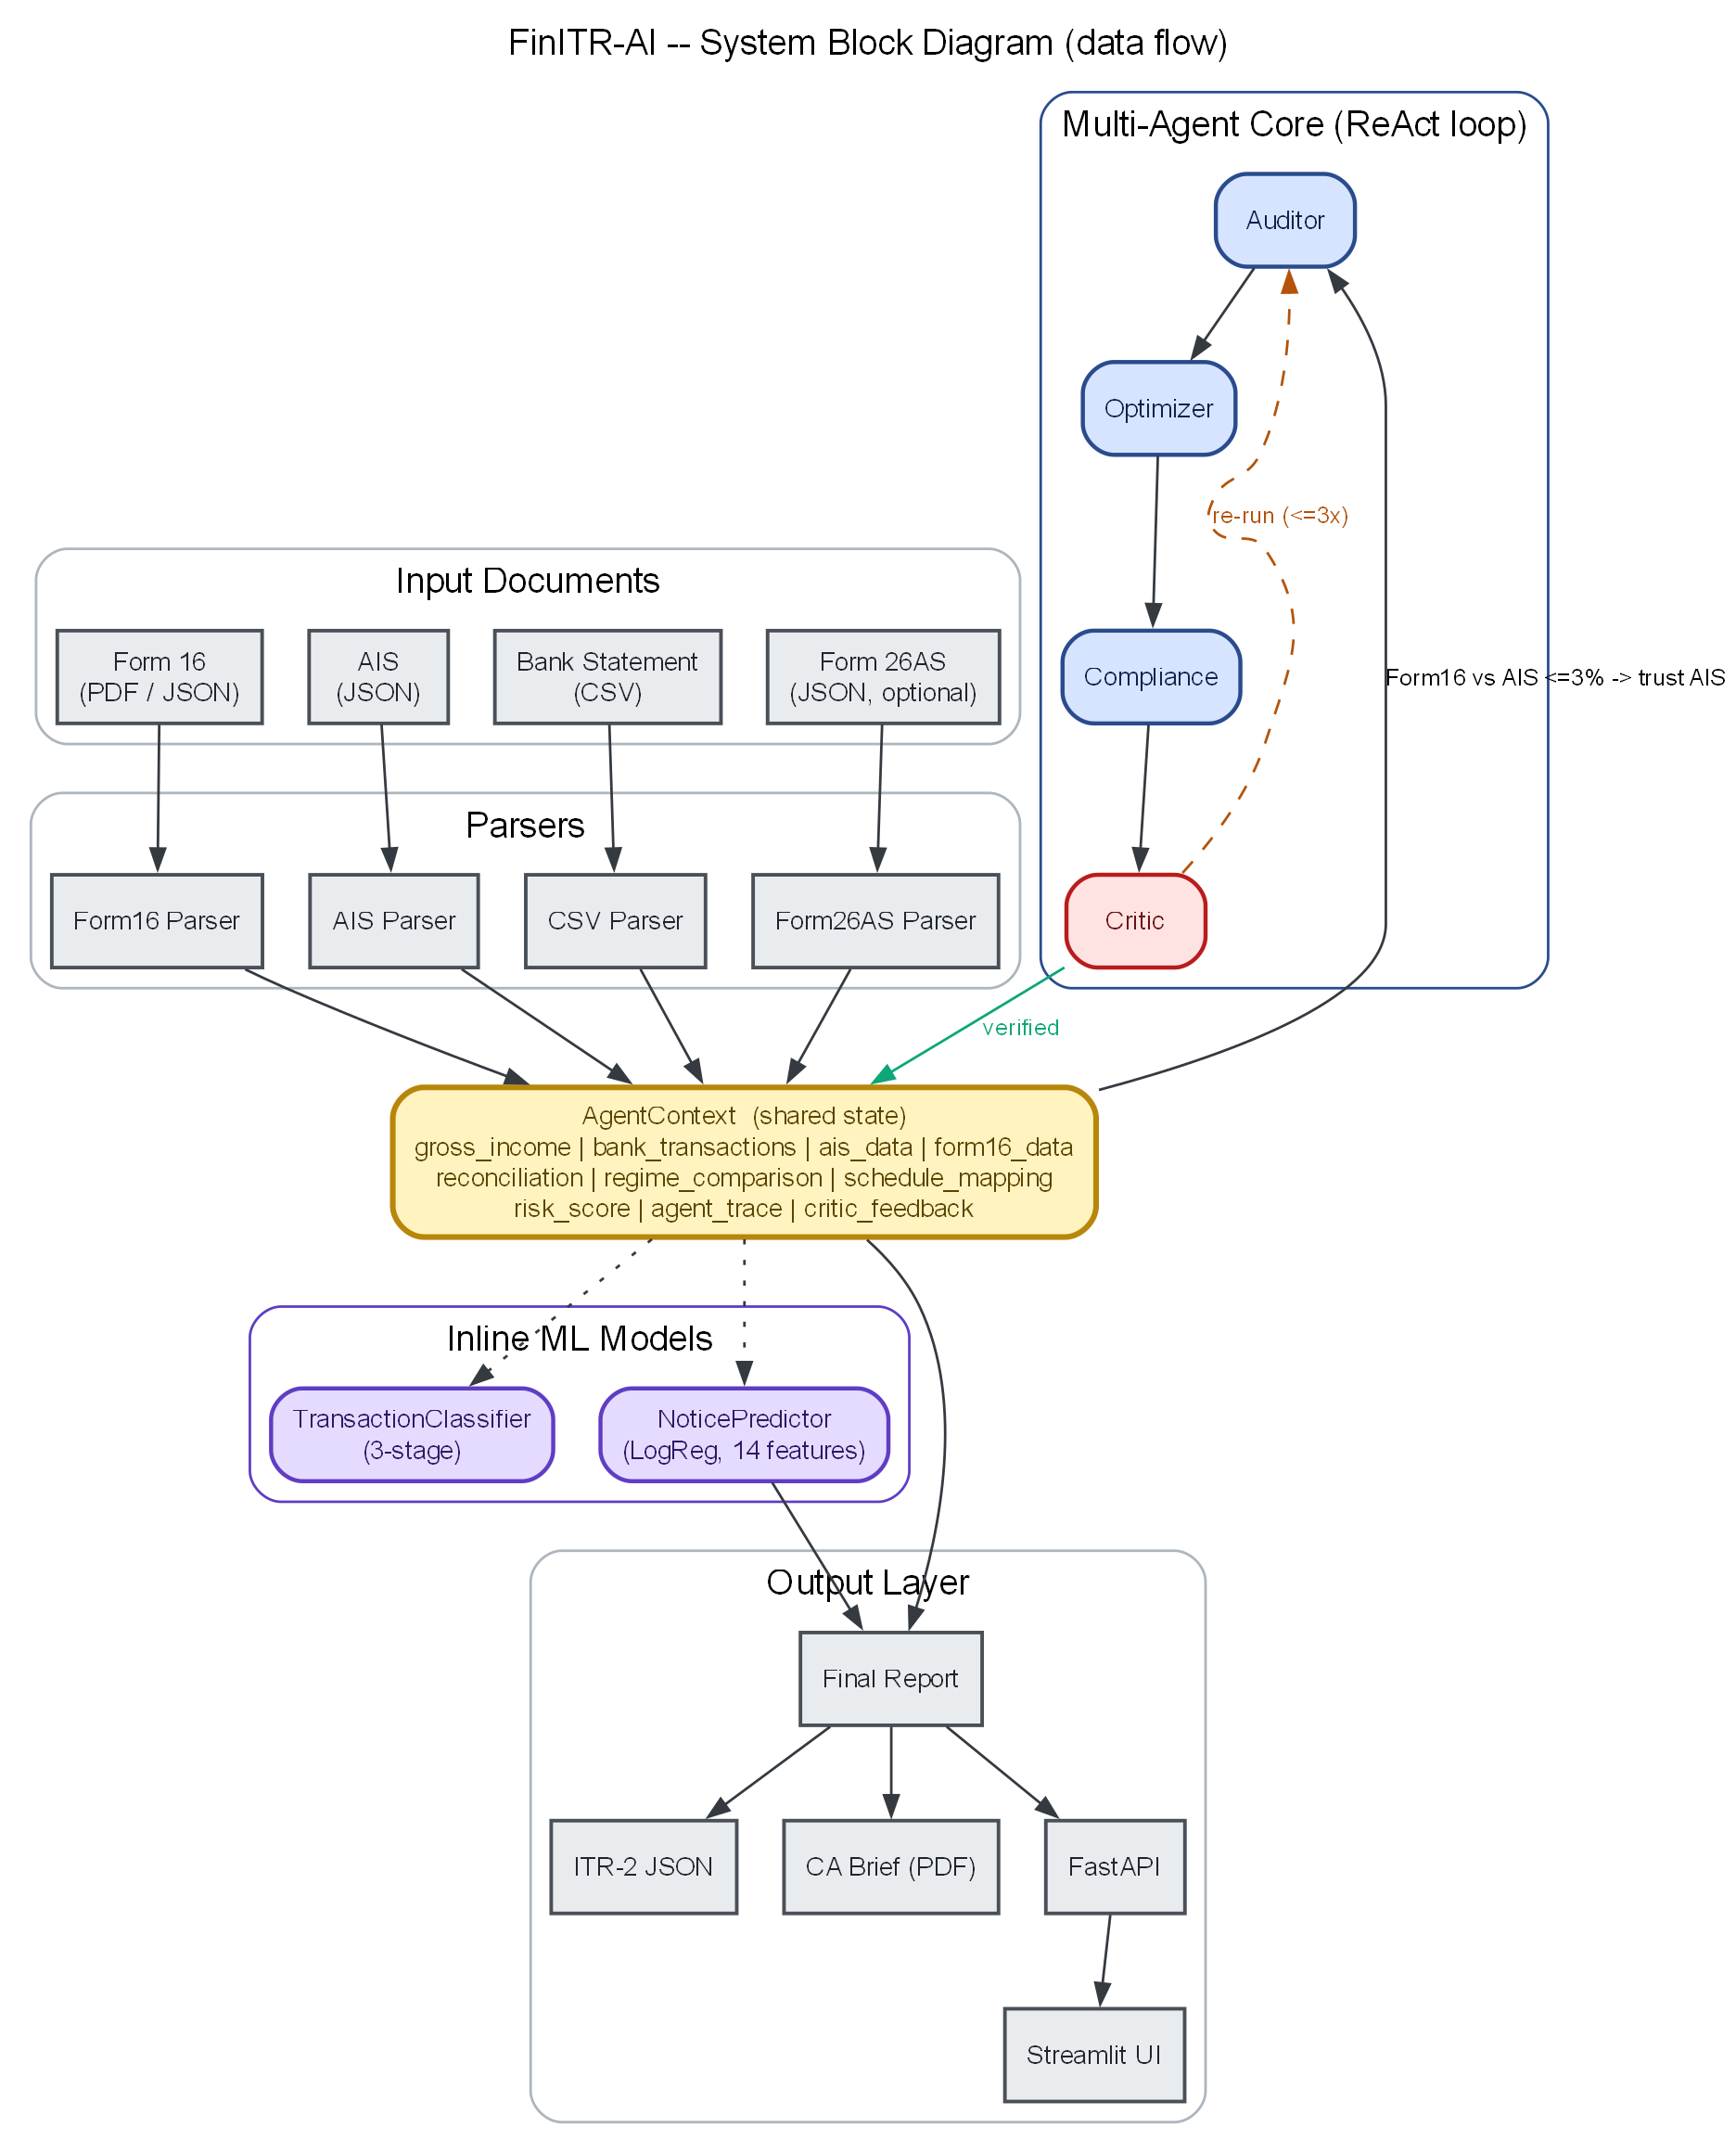
\includegraphics[width=0.9\textwidth]{images/block_diagram.png}
    \caption{System block diagram --- document ingestion, the shared AgentContext, the four-agent core, the inline ML models, and the output layer.}
    \label{fig:block-diagram}
\end{figure}

The pivot of the whole design is the shared data model, the \texttt{AgentContext}.
It is a single mutable record that every component reads from and writes to, and
it is what allows the agents to cooperate without passing tangled arguments
around. Its principal fields are the following:

\begin{itemize}
    \item the parsed document inputs --- \texttt{bank\_transactions},
          \texttt{form16\_data}, \texttt{ais\_data}, \texttt{form26as\_data};
    \item the accumulated agent outputs --- \texttt{reconciliation} and
          \texttt{anomalies} and \texttt{risk\_score} from the Auditor,
          \texttt{regime\_comparison} and \texttt{ctc\_strategy} from the
          Optimizer, \texttt{itr\_form\_recommendation} and
          \texttt{schedule\_mapping} from the Compliance agent, and
          \texttt{verification\_results} from the Critic;
    \item the user profile --- \texttt{gross\_income}, \texttt{basic\_salary},
          \texttt{employer\_nps}, and the \texttt{assessment\_year}; and
    \item the orchestrator's own bookkeeping --- the current \texttt{iteration},
          the \texttt{max\_iterations} bound, the running \texttt{agent\_trace},
          and the \texttt{critic\_feedback} list that carries blocked claims
          between iterations.
\end{itemize}

A small but important piece of robustness lives at the parsing boundary. Real
documents are noisy: a Form 16 produced by optical character recognition will
often disagree with the AIS by a few rupees because of rounding. The
orchestrator absorbs this rather than propagating it. When the Form 16 gross
salary and the AIS salary differ by no more than three percent, it treats the
difference as noise and adopts the AIS figure as ground truth, scaling the basic
salary proportionally. The logic is shown below.

\algname{reconcile\_gross\_income(form16, ais)}
\begin{lstlisting}[style=pseudo]
PROCEDURE reconcile_gross_income(form16, ais):
    f16_gross <- form16.gross_salary
    ais_salary <- sum(e.amount for e in ais.sft_entries
                                 if e.type == "salary")
    IF ais_salary > 0 AND
       |f16_gross - ais_salary| <= 0.03 * ais_salary THEN
        gross_income <- ais_salary          # trust AIS
        IF form16.basic > 0 AND f16_gross > 0 THEN
            basic <- round(form16.basic * (ais_salary / f16_gross))
        ELSE
            basic <- 0.40 * ais_salary
    ELSE
        gross_income <- f16_gross            # genuine mismatch: keep both
        basic <- form16.basic OR 0.40 * f16_gross
    RETURN gross_income, basic
\end{lstlisting}

The decision to trust the AIS within the tolerance, rather than the
employer-issued Form 16, follows from the asymmetry described in
Chapter~\ref{chap:introduction}: the department's record is the one against
which the return is matched, so where the two nearly agree, aligning to the AIS
removes a spurious mismatch before it can inflate the risk score.

\section{Architecture and the ReAct Control Loop}
\label{sec:architecture}

The architecture, shown in Figure~\ref{fig:architecture}, is driven by the
orchestrator. Every agent is a subclass of a common base that provides timing,
tool access, and a uniform result structure, so the orchestrator can treat them
interchangeably and record, for each one, its status, its duration, the tools it
called, and any warnings it raised.

\begin{figure}[H]
    \centering
    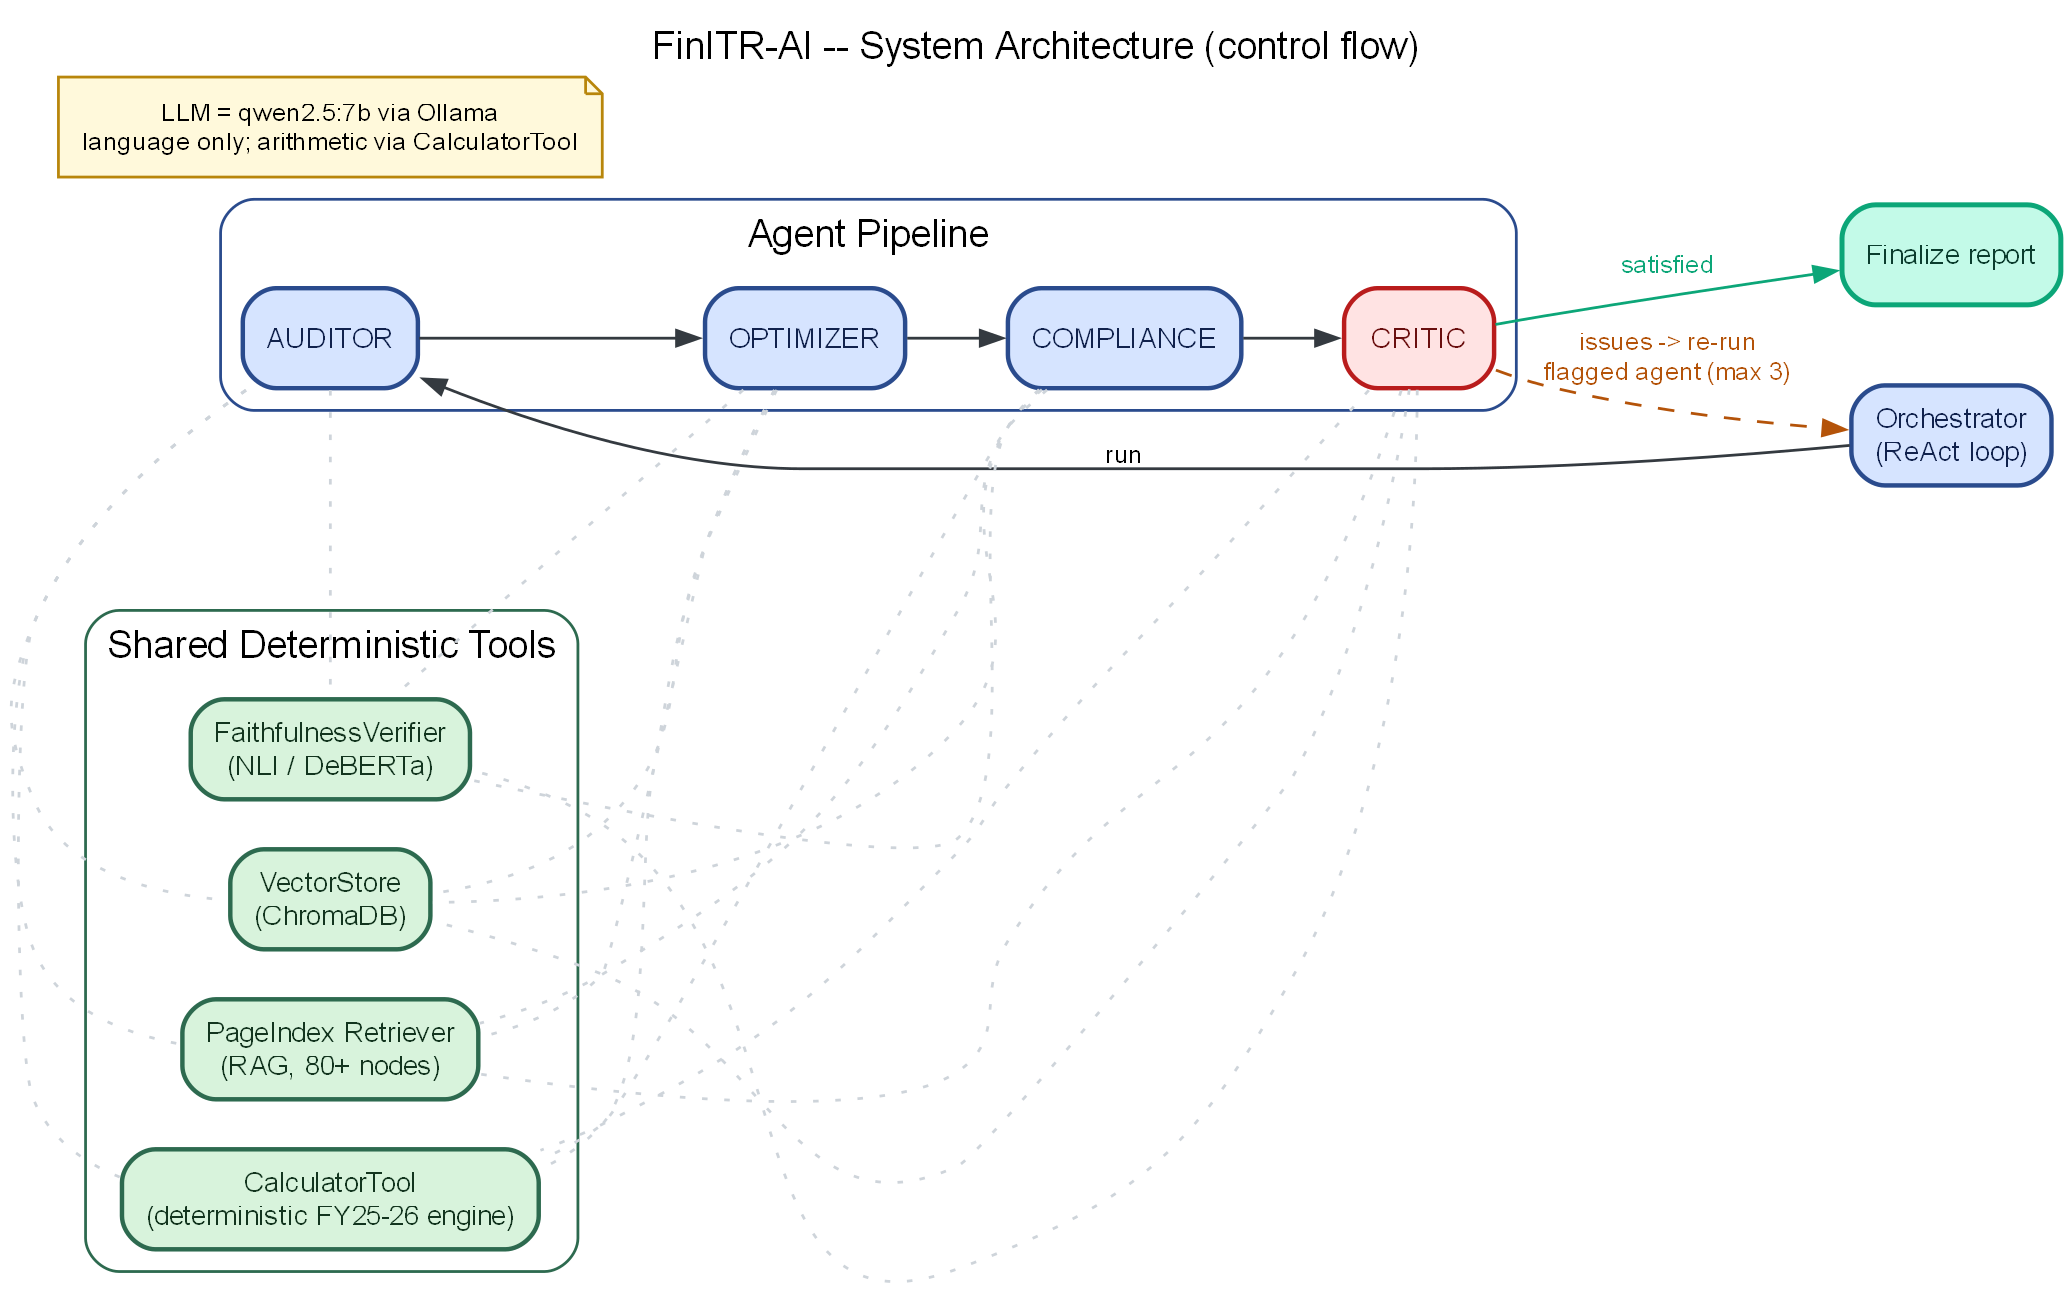
\includegraphics[width=0.9\textwidth]{images/architecture.png}
    \caption{System architecture --- the ReAct orchestrator, the four agents, the shared deterministic tools, and the critic re-run loop.}
    \label{fig:architecture}
\end{figure}

The control loop itself is intentionally simple, and its bounded nature is a
deliberate safeguard against the kind of runaway self-correction that
multi-agent systems can fall into. On the first pass all three working agents
run and the Critic reviews. If the Critic is satisfied, the report is finalised.
If not, the Critic's feedback names the offending agent and the specific claims
it blocked; the orchestrator re-runs only that agent, with the constraints
attached to the context, and then re-runs the Critic. This continues for at most
three iterations. The full procedure is given below.

\algname{orchestrate(documents) \quad / \quad should\_rerun(agent\_name, ctx)}
\begin{lstlisting}[style=pseudo]
PROCEDURE orchestrate(documents):
    ctx <- new AgentContext
    parse_documents_into(ctx, documents)        # fills ctx inputs
    reconcile_gross_income(ctx)                  # noise tolerance

    iteration <- 0
    WHILE iteration < ctx.max_iterations:
        ctx.iteration <- iteration

        IF iteration == 0 OR should_rerun("auditor", ctx):
            run(Auditor, ctx)                    # writes reconciliation,
                                                 # anomalies, risk_score
        IF iteration == 0 OR should_rerun("optimizer", ctx):
            run(Optimizer, ctx)                  # writes regime_comparison
        IF iteration == 0 OR should_rerun("compliance", ctx):
            run(Compliance, ctx)                 # writes itr_form, schedules

        result <- run(Critic, ctx)               # verifies all claims
        IF result.status == "success":
            BREAK                                # nothing to fix
        ctx.critic_feedback.append({
            issues: result.warnings,
            blocked_claims: result.blocked_claims
        })
        iteration <- iteration + 1

    report <- build_report(ctx)
    report.notice_prediction <- NoticePredictor.predict(report)
    RETURN report

PROCEDURE should_rerun(agent_name, ctx):
    # re-run an agent only if the latest critic feedback
    # names it as the source of an issue or a blocked claim
    latest <- ctx.critic_feedback.last
    RETURN any(agent_name in issue.source
               for issue in latest.issues)
        OR any(agent_name in claim.source
               for claim in latest.blocked_claims)
\end{lstlisting}

After the loop terminates, two machine-learning models annotate the report. The
transaction classifier has already done its work inside the Auditor; the
standalone notice predictor now estimates the probability of a Section 143(1)
notice from features of the finished report. Both are described in the module
sections that follow.

\subsection{A Worked Example}
It helps to fix ideas with a concrete trace before dissecting each agent.
Consider a salaried filer with a gross salary of about Rs.~18,50,000 declared on
Form 16, whose AIS additionally contains a fixed-deposit interest entry of
Rs.~42,000 (reported under SFT but absent from Form 16) and an equity-sale
proceed of Rs.~1,20,000 routed through a broker, with a matching credit visible
in the bank statement. The pipeline proceeds as follows. The Auditor classifies
the bank credits, finds the FD interest and the equity sale in the AIS but not
in Form 16, records them in the reconciliation ledger as \texttt{ais\_only}
items, and scores the resulting notice risk. The Optimizer computes the tax both
ways; under the New Regime the standard deduction of Rs.~75,000 brings taxable
income to Rs.~17,75,000, and the slab computation (described in
Section~\ref{sec:module-two}) yields a slab tax near Rs.~1,55,000 to which the
four percent cess adds roughly Rs.~6,200, for a liability of about
Rs.~1,61,200; the Old Regime, lacking enough deductions to overcome its higher
rates, comes out higher, so the New Regime is recommended. The Compliance agent
sees a capital-gains signal and therefore selects ITR-2, mapping the equity sale
to Schedule CG and the interest to Schedule OS. The Critic verifies that no
disallowed deduction was claimed under the New Regime and that each cited section
exists, and the notice predictor, seeing AIS income not present in Form 16,
returns an elevated probability. We return to the individual steps below.

\section{Module One -- Auditor Agent}
\label{sec:module-one}

The Auditor is the entry point and, in many ways, the core contribution of the
system. Its responsibility is reconciliation and risk. Its overall workflow,
shown in Figure~\ref{fig:module1}, has six steps: extract income items from each
of the three sources, merge them into a unified ledger, cross-reference the AIS
against Form 16, detect anomalies in the bank statement, compute a risk score
from the evidence, and generate targeted interview questions for the items that
need human input.

\begin{figure}[H]
    \centering
    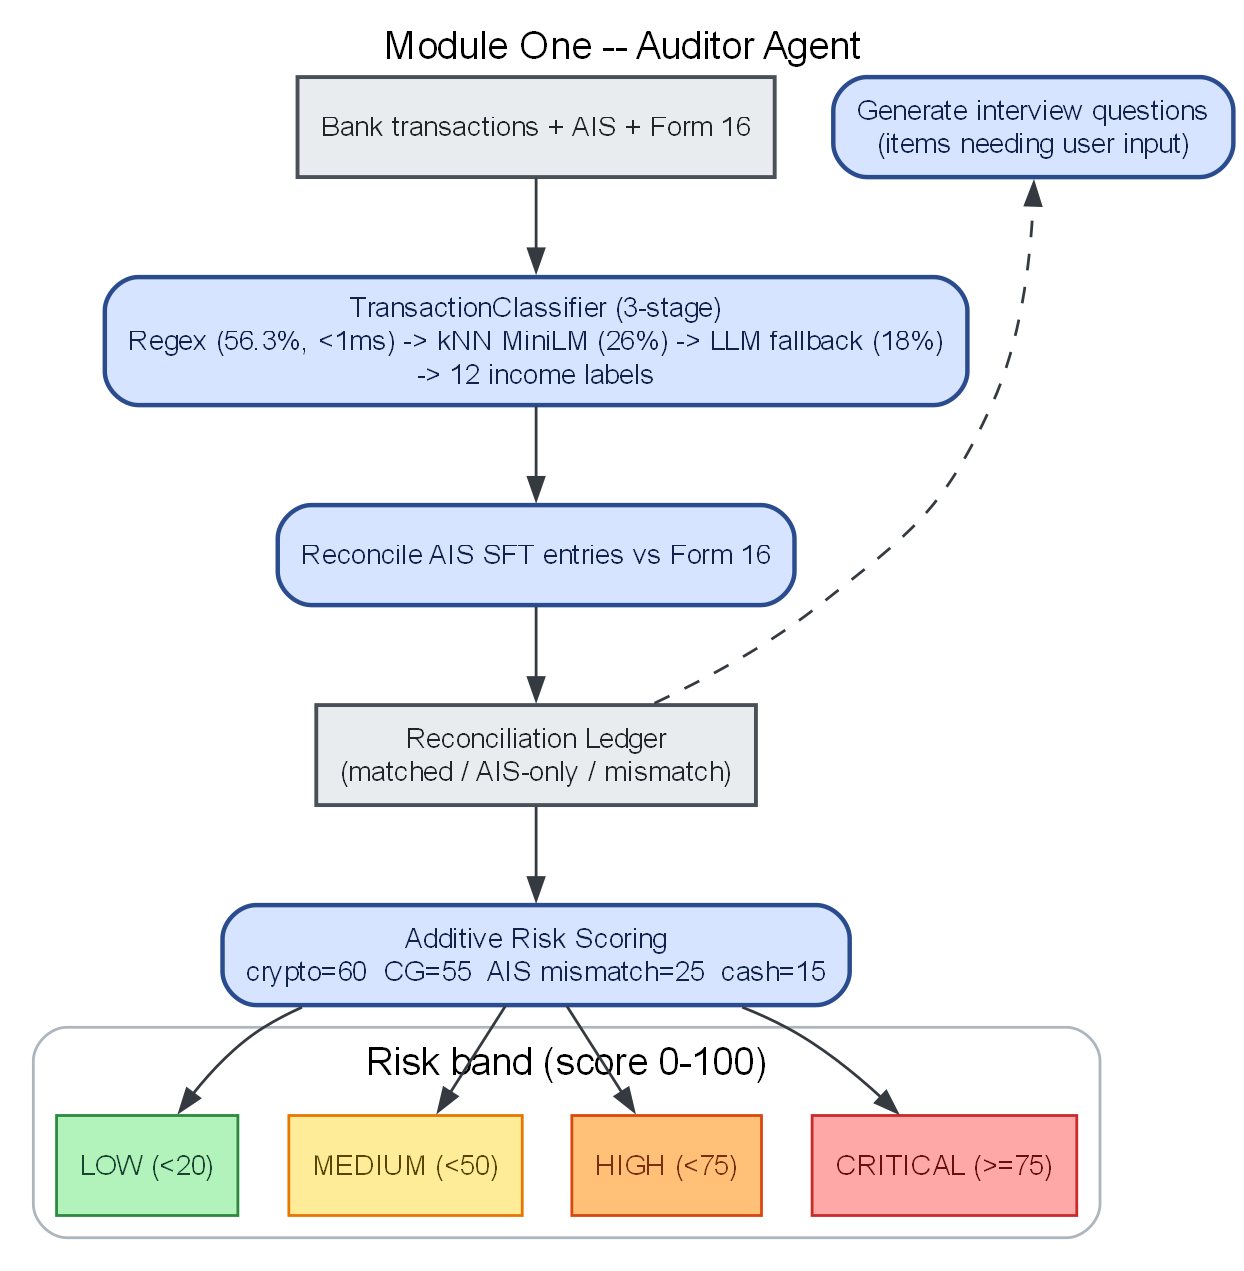
\includegraphics[width=0.9\textwidth]{images/module1_flow.png}
    \caption{Auditor Agent --- transaction classification, AIS-versus-Form-16 reconciliation, and additive risk scoring.}
    \label{fig:module1}
\end{figure}

\subsection{The Three-Stage Transaction Classifier}
Before reconciliation can begin, every bank credit must be assigned an income
type. This is harder than it sounds, because real Indian bank statements are
written in a terse, inconsistent shorthand --- transfer codes, UTR references,
truncated merchant names, and Hinglish vendors such as ``Aman Juicewala'' or
``Sharma Sweet Mart''. The classifier addresses this with a three-stage cascade
that trades speed for coverage: cheap rules first, learned similarity next, and
the language model only as a last resort. The taxonomy has twelve labels, each
carrying a tax-relevance flag and an ITR schedule.

\algname{classify\_transaction(description, direction)}
\begin{lstlisting}[style=pseudo]
PROCEDURE classify_transaction(description, direction):
    cleaned <- normalize(description, direction)   # strip codes/refs

    # Stage 1 -- high-precision regex (resolves the majority,
    #            sub-millisecond, no model loaded)
    FOR (pattern, label, confidence) IN PATTERN_RULES:
        IF pattern matches cleaned OR description:
            RETURN result(label, confidence, stage="pattern")

    # Stage 2 -- kNN over multilingual MiniLM embeddings
    q <- embed(cleaned)                            # 384-dim vector
    sims <- cosine(q, train_embeddings)            # vs labelled set
    top_k <- argsort(sims)[-k:]                    # k = 5
    label <- majority_vote(train_labels[top_k])
    confidence <- mean(sims of winning label)
    IF confidence >= 0.65:
        RETURN result(label, confidence, stage="ml")

    # Stage 3 -- LLM fallback for the genuinely ambiguous remainder
    llm <- ask_local_llm_to_classify(description, cleaned)
    IF llm is valid:
        RETURN result(llm.label, llm.confidence, stage="llm")

    RETURN result(label, confidence, stage="ml_low_conf")
\end{lstlisting}

The ordering is the point. Stage one disposes of the unambiguous majority --- a
line containing ``WAZIRX'' is crypto, a line containing ``SALARY'' is salary ---
at essentially no cost. Stage two handles the noisy middle, where a multilingual
sentence embedding places ``Sharma Sweet Mart'' near other small-merchant
expenses even though no rule names it. Stage three, the only stage that invokes
the model, is reached by a small fraction of transactions, which keeps the
pipeline fast and keeps the model away from decisions a rule can make more
reliably. Every income-critical label --- capital market, crypto, interest,
dividend, freelance --- is one the rules and the embeddings handle with high
precision, so the costly stage is rarely the one deciding a taxable item.

\subsection{Reconciliation and the Unified Ledger}
With the bank credits classified, the Auditor extracts income items from all
three sources and merges them. Salary is matched across Form 16, the AIS, and
the bank; a difference below Rs.~100 is treated as confirmed, anything larger as
a mismatch. Every non-salary AIS entry is then checked against the bank and,
critically, against Form 16: an item the government reports but the employer's
Form 16 does not contain is exactly the kind of undeclared income that triggers
a notice, and it is recorded as an \texttt{ais\_only} item with a risk weight
attached. Bank credits that appear in neither Form 16 nor the AIS are recorded
too, but at a low weight, because the government does not yet know about them.

\subsection{Evidence-Weighted Risk Scoring}
The risk score is deliberately not a black box. It is an additive sum of
evidence-based weights, each chosen to reflect how strongly a given signal
predicts a notice, and then banded into four levels. The weights encode genuine
tax knowledge: undeclared crypto scores highest because the 194S TDS makes
non-disclosure almost certain to be caught; undeclared capital gains score
nearly as high because SEBI and STT data give the department full visibility; an
AIS-versus-Form-16 mismatch scores in the middle; a large cash deposit scores
lower.

\algname{compute\_risk(mismatches, anomalies) \quad with evidence WEIGHTS}
\begin{lstlisting}[style=pseudo]
WEIGHTS = { crypto_undeclared: 60, capital_gains_undeclared: 55,
            ais_mismatch_income: 25, freelance_undeclared: 25,
            property_unreported: 20, high_value_cash: 15,
            savings_interest_missing: 10 }

PROCEDURE compute_risk(mismatches, anomalies):
    total <- 0
    FOR m IN mismatches:
        total <- total + WEIGHTS[m.type]
    FOR a IN anomalies:
        IF a.in_ais:                  # already counted via mismatch
            CONTINUE                  # avoid double counting
        total <- total + a.risk_weight
    score <- min(100, total)
    IF   score < 20: level <- "LOW"
    ELIF score < 50: level <- "MEDIUM"
    ELIF score < 75: level <- "HIGH"
    ELSE:            level <- "CRITICAL"
    RETURN { score, level, breakdown }
\end{lstlisting}

The double-counting guard matters: an item that appears both as an AIS mismatch
and as a bank anomaly is counted once, not twice, so the score reflects distinct
pieces of evidence rather than the same fact seen from two angles. The banding
is intentionally conservative on the side of caution --- the design philosophy,
developed further in Chapter~\ref{chap:challenges}, is that a missed risk costs
the user money while an over-flag costs only a second look, so the thresholds
are set so that a genuine high-risk case is never quietly scored low.

\section{Module Two -- Optimizer Agent}
\label{sec:module-two}

The Optimizer answers the two questions a filer most wants answered: how much
tax, and under which regime. Its workflow, in Figure~\ref{fig:module2}, gathers
the applicable deductions, computes the liability under both regimes through the
CalculatorTool, compares them, and adds a CTC-restructuring analysis, finishing
with a natural-language explanation generated by the local model.

\begin{figure}[H]
    \centering
    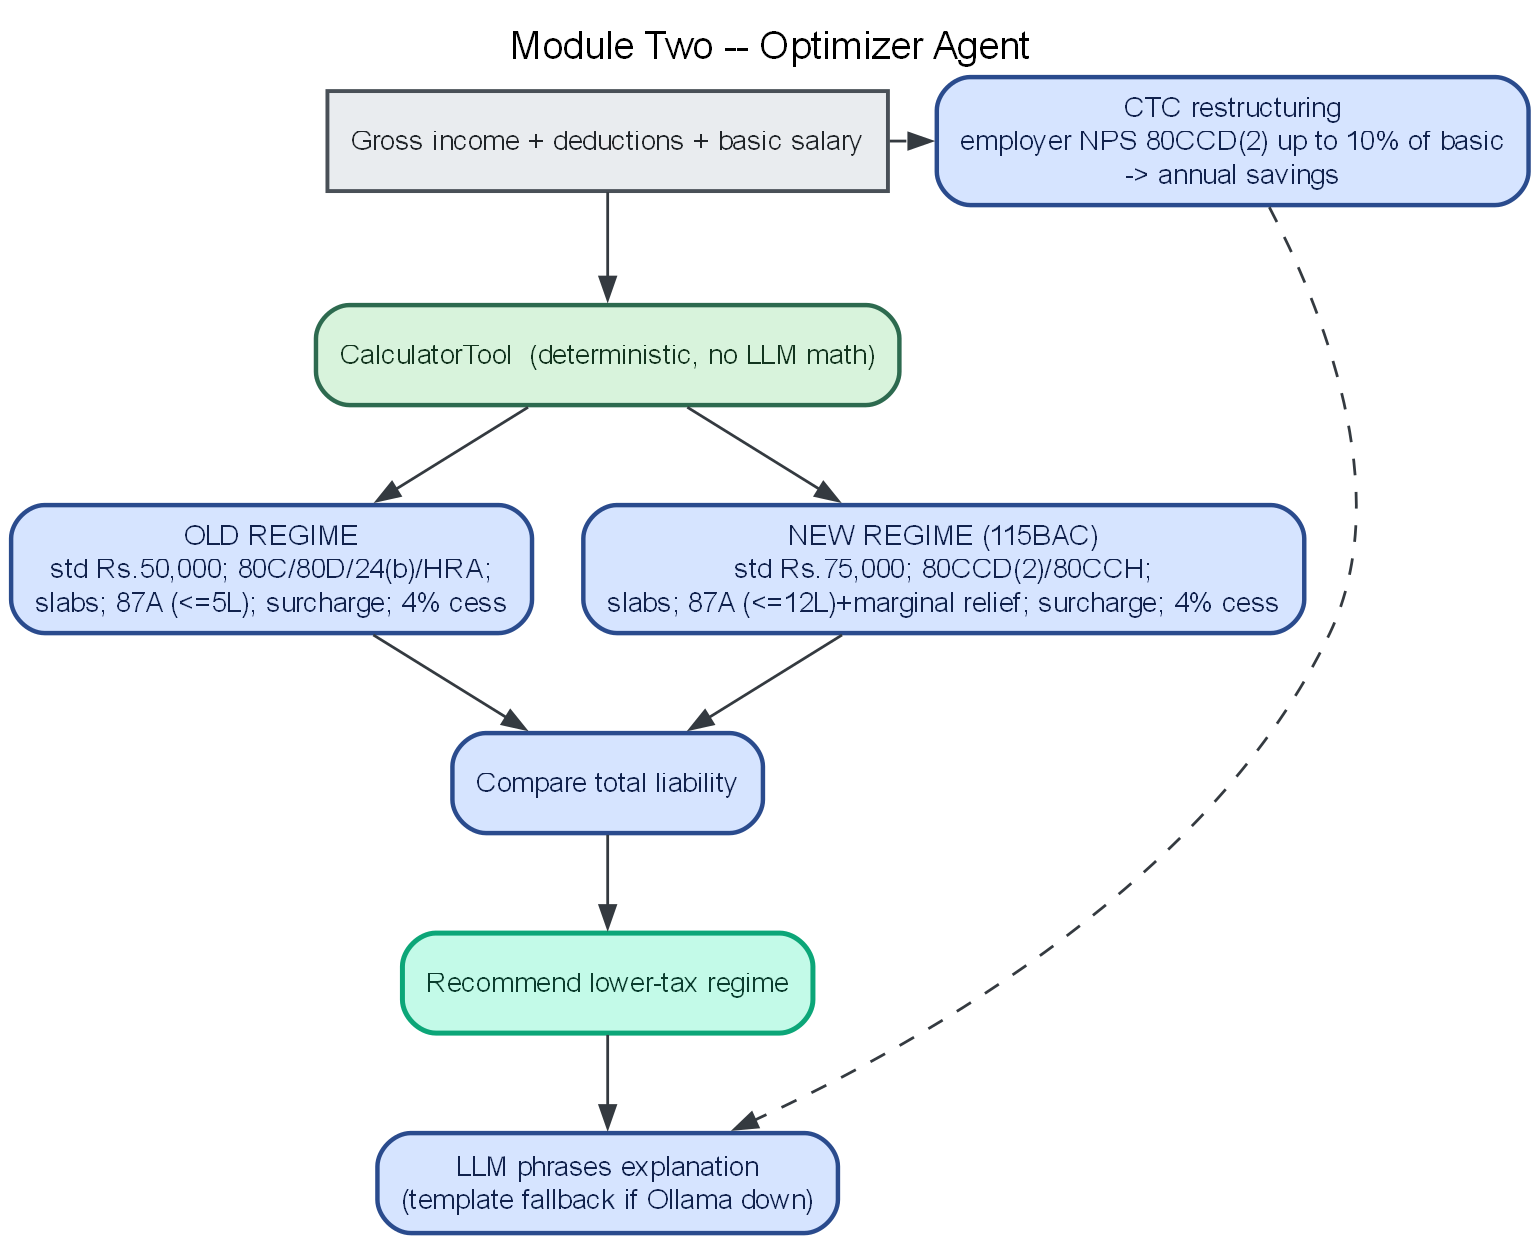
\includegraphics[width=0.9\textwidth]{images/module2_flow.png}
    \caption{Optimizer Agent --- dual-regime computation via the deterministic engine, deduction and NPS optimisation, and regime recommendation.}
    \label{fig:module2}
\end{figure}

\subsection{The Deterministic Slab Engine}
The heart of the Optimizer --- and, by the ablation in
Chapter~\ref{chap:results}, the most important single component in the whole
system --- is the deterministic tax engine. It walks the slab structure for the
chosen regime, accumulating tax band by band. The same routine serves both
regimes; only the slab table, the standard deduction, and the rebate parameters
differ.

\algname{slab\_tax(taxable\_income, slabs) \quad / \quad new\_regime\_tax(gross, deductions)}
\begin{lstlisting}[style=pseudo]
PROCEDURE slab_tax(taxable_income, slabs):
    tax <- 0 ; remaining <- taxable_income
    FOR (lo, hi, rate) IN slabs:
        IF remaining <= 0: BREAK
        width <- (hi - lo + 1) IF hi != INF ELSE remaining
        in_band <- min(remaining, width)
        tax <- tax + in_band * rate
        remaining <- remaining - in_band
    RETURN round(tax, 2)

PROCEDURE new_regime_tax(gross, deductions):
    std <- min(75000, gross)             # FY25-26 new-regime std deduction
    allowed <- deductions.80CCD_2 + deductions.80CCH   # only these two
    taxable <- max(0, gross - std - allowed)
    base <- slab_tax(taxable, NEW_SLABS)

    # Section 87A rebate + marginal-relief zone
    rebate <- 0 ; relief <- FALSE
    IF taxable <= 1200000:
        rebate <- min(base, 60000)
    ELIF taxable <= 1275000:                 # marginal relief band
        excess <- taxable - 1200000
        IF base > excess:
            rebate <- base - excess ; relief <- TRUE

    after_rebate <- max(0, base - rebate)
    surcharge <- compute_surcharge(after_rebate, taxable, "new")
    cess <- 0.04 * (after_rebate + surcharge)
    RETURN after_rebate + surcharge + cess
\end{lstlisting}

Two subtleties are worth drawing out, because they are exactly the points at
which the general models in our benchmark fail. The first is the marginal-relief
band between Rs.~12,00,000 and roughly Rs.~12,75,000: inside it, the rebate is
not all-or-nothing but is tapered so that the tax never exceeds the income earned
above the twelve-lakh threshold. The second is the four percent cess, which is
applied to the sum of tax and surcharge, not to the base tax alone --- a step
the models routinely omit. The Old Regime routine mirrors this structure but
caps each Chapter VI-A deduction at its statutory limit (80C at Rs.~1,50,000,
24(b) at Rs.~2,00,000, and so on) before computing the slab tax against the
lower, deduction-friendly Old Regime slabs.

\subsection{HRA, Surcharge, and CTC Restructuring}
The HRA exemption under Section 10(13A) is computed as the statutory minimum of
three quantities, which is one of the places a naive implementation tends to
take only one of the three:

\algname{hra\_exemption(basic, hra\_received, rent\_paid, metro)}
\begin{lstlisting}[style=pseudo]
PROCEDURE hra_exemption(basic, hra_received, rent_paid, metro):
    IF rent_paid <= 0 OR hra_received <= 0: RETURN 0
    option1 <- hra_received
    option2 <- basic * (0.50 IF metro ELSE 0.40)
    option3 <- max(0, rent_paid - 0.10 * basic)
    RETURN min(option1, option2, option3)
\end{lstlisting}

The surcharge routine applies the appropriate rate band by total income and then
applies marginal relief so that the surcharge cannot push the total above the
income earned past the threshold. Finally, the CTC-restructuring analysis models
a concrete, lawful saving available even under the New Regime: an employer NPS
contribution under Section 80CCD(2), deductible up to ten percent of basic
salary. The Optimizer computes the tax with and without the maximum employer NPS
and reports the difference as an annual saving the user can ask their employer to
realise. The regime comparison itself is a straightforward selection of the
lower liability, but because both figures come from the deterministic engine, the
comparison is trustworthy in a way a model's self-reported numbers are not. The
language model is then asked only to phrase the recommendation, with an explicit
instruction not to compute anything; if the local model is unavailable, a
template fills in, so the numbers never depend on the model running at all.

\section{Module Three -- Compliance Agent}
\label{sec:module-three}

The Compliance agent decides which ITR form the filer must use and maps each
income item to its schedule. Its workflow, in Figure~\ref{fig:module3}, first
classifies the income types present, then applies the form-eligibility rules,
then maps schedules using document signals.

\begin{figure}[H]
    \centering
    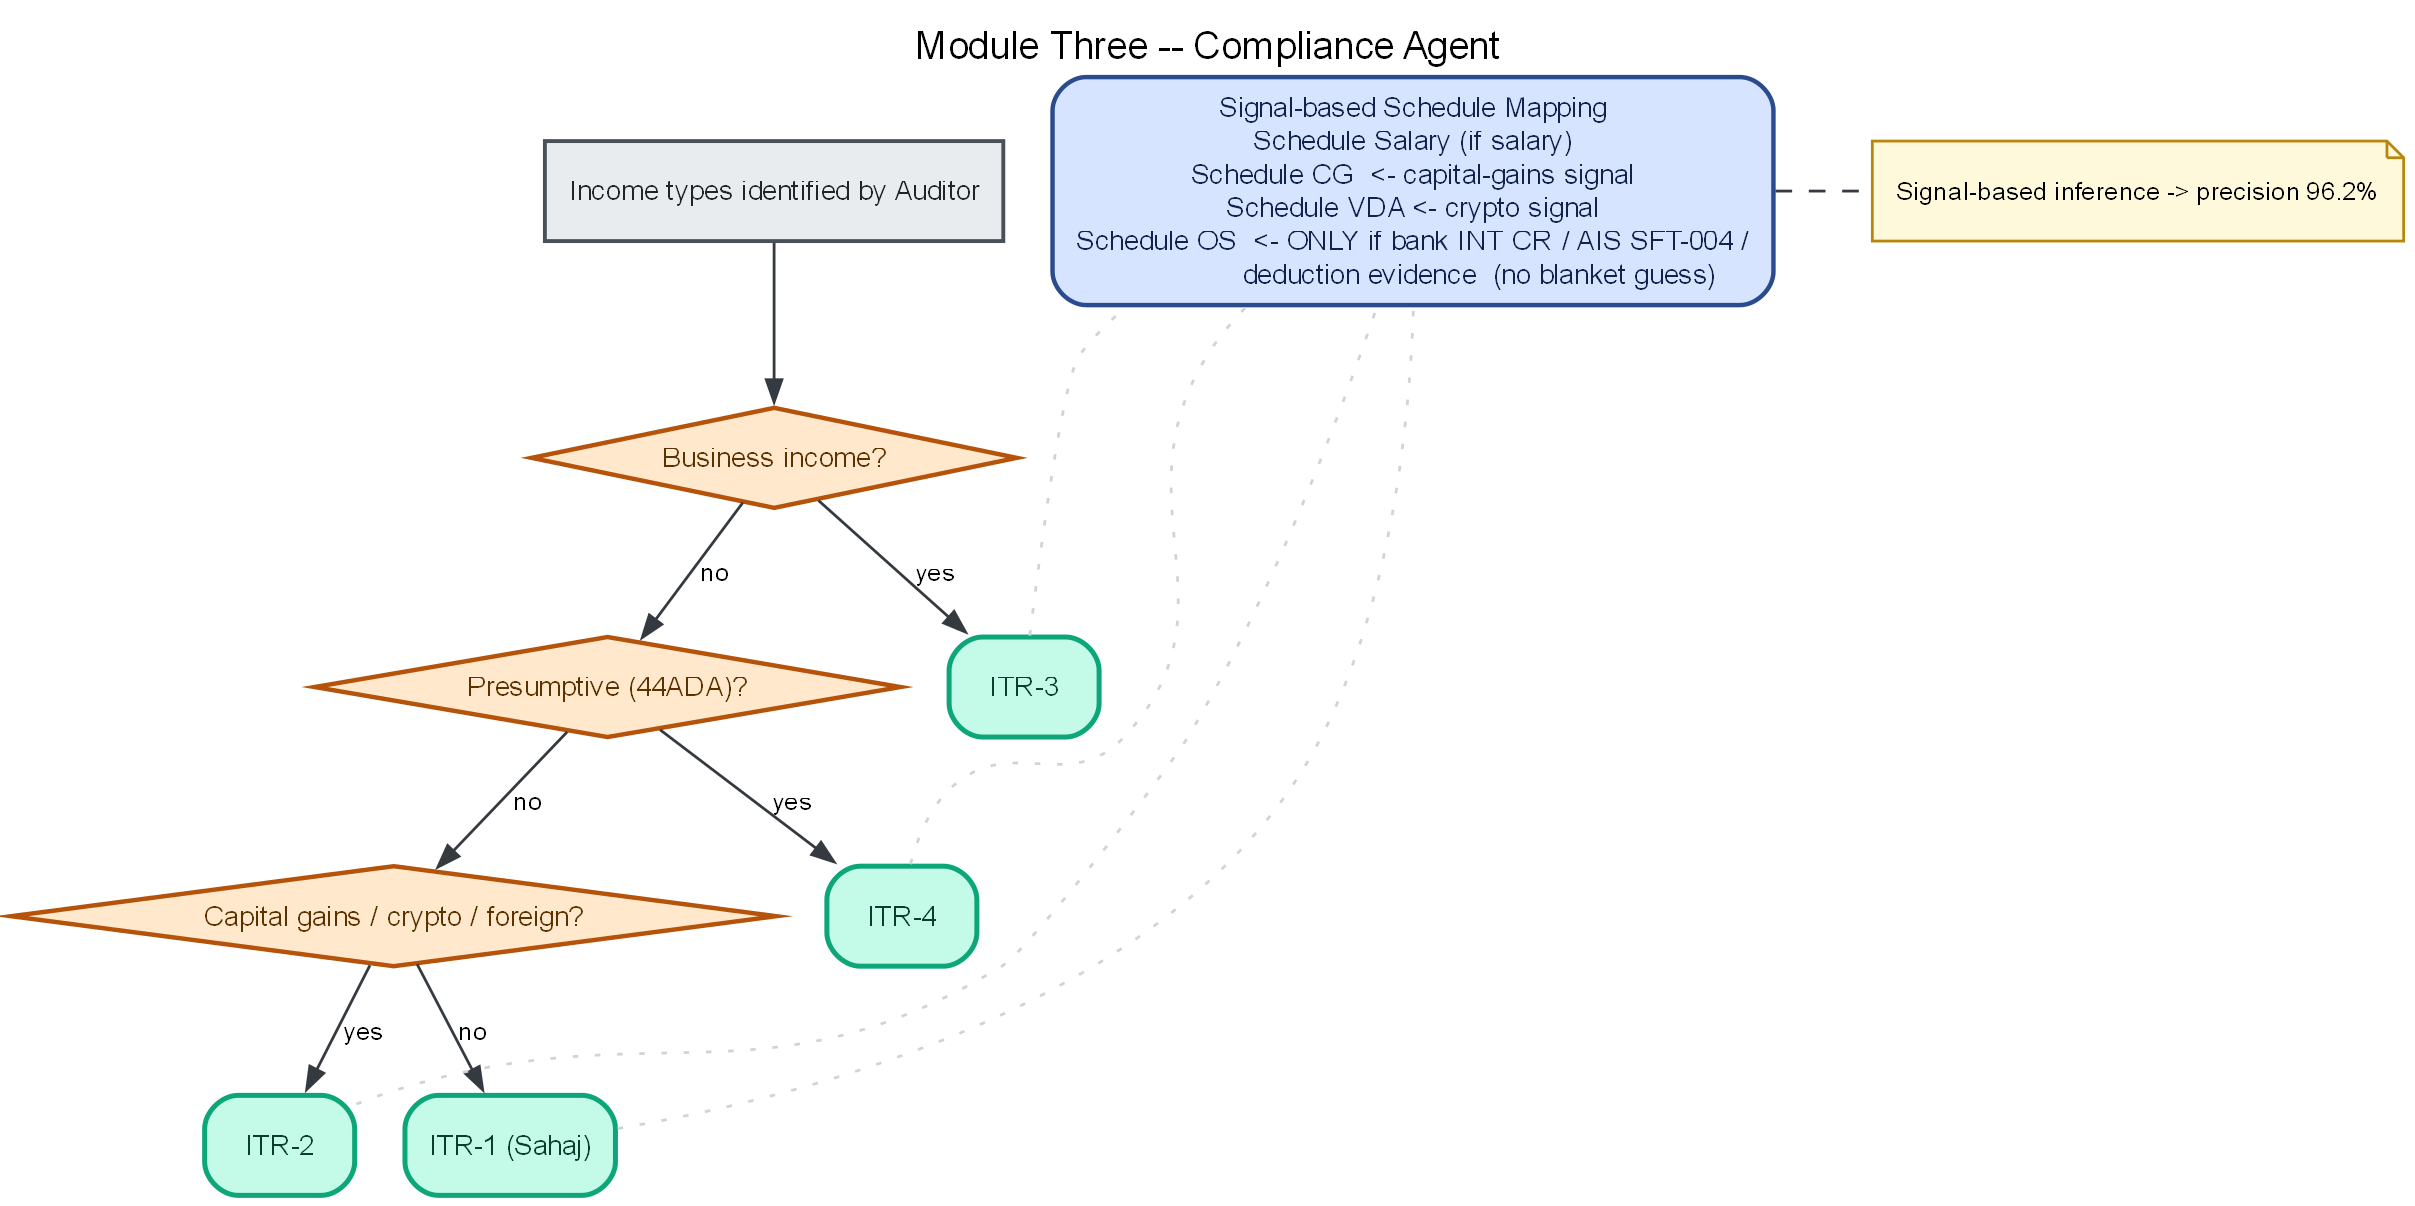
\includegraphics[width=0.9\textwidth]{images/module3_flow.png}
    \caption{Compliance Agent --- ITR form selection and signal-based schedule mapping.}
    \label{fig:module3}
\end{figure}

\subsection{Form Selection as a Blocker Cascade}
ITR form selection is expressed not as a positive lookup but as a process of
elimination, which mirrors how the rules actually work: each form is disqualified
by the presence of certain income types, and the simplest surviving form is
chosen.

\algname{select\_itr\_form(income\_types)}
\begin{lstlisting}[style=pseudo]
PROCEDURE select_itr_form(income_types):
    # each form lists the income types that DISQUALIFY it
    blocked <- {}
    FOR form IN [ITR-1, ITR-2, ITR-4]:
        hits <- [t for t in RULES[form].blocked_by
                          if t in income_types]
        IF hits: blocked[form] <- hits

    IF "ITR-1" not in blocked AND
       ("salary" in income_types OR
        "other_sources" in income_types):
        RETURN "ITR-1"        # simplest case: salary/interest <= 50L
    ELIF "business_income" in income_types:
        RETURN ("ITR-4" if "ITR-4" not in blocked else "ITR-3")
    ELIF "ITR-2" not in blocked:
        RETURN "ITR-2"        # capital gains / crypto / foreign
    ELSE:
        RETURN "ITR-3"        # everything else
\end{lstlisting}

Capital gains or crypto, for instance, appear in the \texttt{blocked\_by} list
of both ITR-1 and ITR-4, so their presence forces the filer up to ITR-2 ---
which is precisely why the worked example earlier landed on ITR-2 the moment an
equity sale was detected.

\subsection{Signal-Based Schedule Inference}
The schedule mapping embodies one of the project's firmest design commitments:
a schedule is asserted only when a document actually supports it. This is most
visible in the handling of Schedule OS (income from other sources), which a less
careful system would attach to almost everyone. Here it is added only on a
concrete signal --- a bank interest credit, an AIS SFT-004 entry, an
old-regime Form 16 carrying deductions that imply interest-bearing investments,
or the presence of capital-gains or crypto activity that makes savings interest
an overwhelming empirical likelihood. The trade-off is explicit and intentional:
this keeps schedule precision very high at the cost of some recall, and the
reasoning is that asserting a schedule the documents do not support is a worse
error, for a filing tool, than omitting one the documents are silent about.
Where a broker or exchange CSV is supplied, the agent goes further and
auto-populates Schedule CG or Schedule VDA with computed gains, set-off, and the
194S TDS credit, drawing on the dedicated schedule builders.

\section{Module Four -- Critic Agent}
\label{sec:module-four}

The Critic is the system's conscience and the mechanism that most distinguishes
it from a prompted model. After the other three agents have run, it collects
every verifiable claim they produced, checks each one along several independent
axes, and either passes it or blocks it. Its workflow is shown in
Figure~\ref{fig:module4}.

\begin{figure}[H]
    \centering
    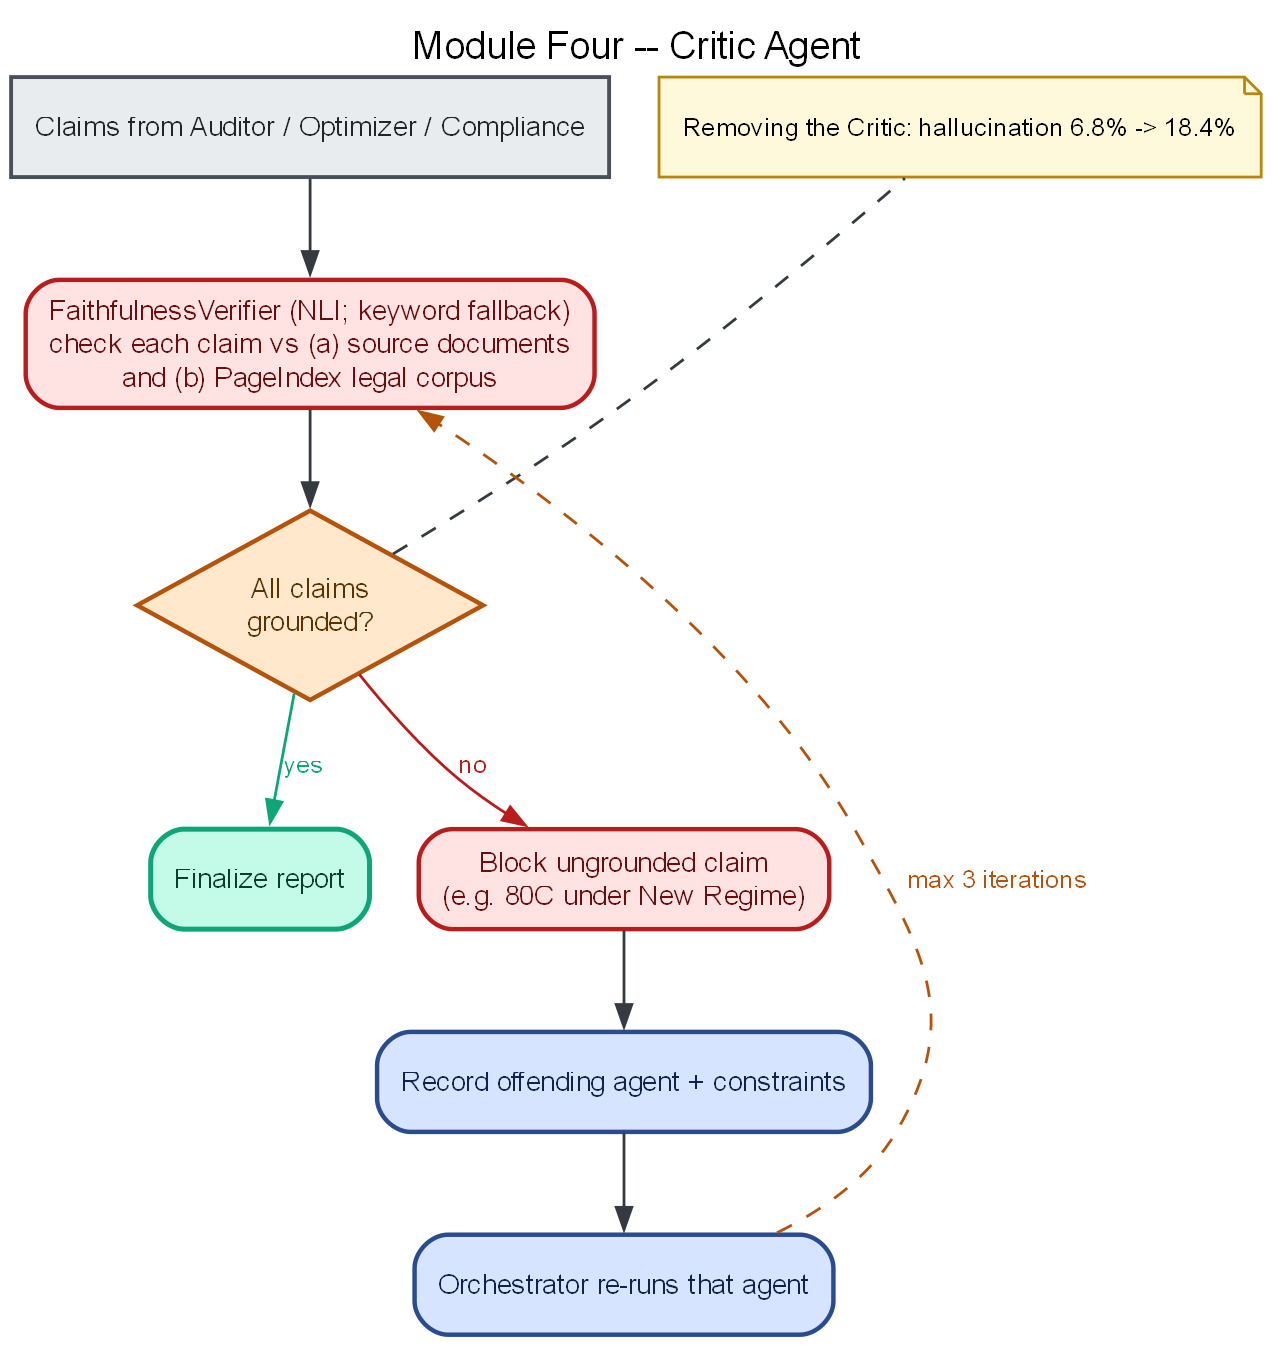
\includegraphics[width=0.9\textwidth]{images/module4_flow.png}
    \caption{Critic Agent --- claim verification against documents and the legal corpus, with the bounded re-run loop.}
    \label{fig:module4}
\end{figure}

\subsection{What Counts as a Claim, and How It Is Checked}
The Critic first assembles claims of several kinds: each deduction the Optimizer
applied (a ``deduction-eligibility'' claim), each legal section the narrative or
the schedule map references (a ``legal-reference'' claim), and each regime's
computed liability (an ``arithmetic'' claim). It then subjects each to up to four
checks.

\algname{verify\_claims(ctx)}
\begin{lstlisting}[style=pseudo]
PROCEDURE verify_claims(ctx):
    blocked <- [] ; verified <- []
    FOR claim IN collect_claims(ctx):

        # Check 1 -- regime compatibility (the classic hallucination)
        IF claim.type == "deduction_eligibility"
           AND ctx.recommended_regime == "new"
           AND normalize(claim.section) IN NEW_REGIME_BLOCKED:
            blocked.append(claim, reason="disallowed under New Regime")
            CONTINUE

        # Check 2 -- the cited section actually exists in the corpus
        IF NOT retriever.section_exists(claim.section):
            IF claim.type == "deduction_eligibility":
                blocked.append(claim, reason="fabricated section")
                CONTINUE

        # Check 3 -- arithmetic re-computation via the calculator
        IF claim.type == "arithmetic":
            recomputed <- calculator.recompute(claim, ctx)
            IF |recomputed - claim.value| > 100:
                warn("arithmetic_mismatch", claim)

        # Check 4 -- NLI faithfulness against retrieved legal text
        evidence <- retriever.retrieve(claim.section).text
        verdict  <- verifier.verify(claim.text, evidence)
        IF verdict.label == "HALLUCINATED":
            blocked.append(claim, reason="NLI contradiction")
        ELSE:
            verified.append(claim)

    status <- "success" IF blocked is empty
                         ELSE "needs_review"
    RETURN status, blocked, verified
\end{lstlisting}

The first check is the one that catches the textbook error --- an 80C, 80D, or
HRA deduction surviving into a New Regime recommendation --- by comparing the
claimed section against an explicit set of provisions the New Regime disallows.
The second guards against invented sections by requiring that the citation
resolve to a real node in the PageIndex corpus. The third independently
re-computes any stated tax figure through the same deterministic engine and
flags a divergence beyond Rs.~100. The fourth is the most general: it retrieves
the authoritative text of the cited section and asks an NLI cross-encoder
whether the claim is actually entailed by that text.

\subsection{The Faithfulness Verifier}
The verifier wraps a DeBERTa-based cross-encoder that scores a (premise,
hypothesis) pair --- here, (retrieved legal text, the claim) --- across the three
NLI labels, mapping entailment to \texttt{FAITHFUL}, contradiction to
\texttt{HALLUCINATED}, and neutral to \texttt{UNVERIFIED}. When the model cannot
be loaded, it degrades gracefully to a keyword-overlap heuristic rather than
failing, so verification still happens, if more crudely, on a minimal install.
The legal text it checks against comes from the PageIndex retriever, a tree-walk
over a hand-built corpus of more than eighty nodes covering both regimes, the
allowed and disallowed deductions, the capital-gains and crypto provisions, the
TDS sections, and the ITR-form rules; a section reference is matched directly to
its node by pattern, and a free-text query falls back to keyword scoring across
the tree. When the Critic blocks a claim, the orchestrator re-runs the
responsible agent --- most often the Optimizer, which then re-gathers deductions
with the blocked section excluded --- and the loop repeats, bounded at three
iterations, until the report is clean. As Chapter~\ref{chap:results} shows, this
single loop is what holds the hallucination rate down to a fraction of what the
same pipeline produces without it.


% ============================================================================
%  CHAPTER 4: CHALLENGES AND SOLUTIONS   (expanded, deep-dive version)
%  Replaces the entire Chapter 4 body in main.tex.
% ============================================================================

\chapter{Challenges and Solutions}
\label{chap:challenges}

Building FinITR-AI was, more than anything, an exercise in working out what the
language model should never be allowed to touch. The recurring discovery was
that the parts of the task a model finds easy --- producing fluent prose,
recognising the rough shape of a problem --- are not the parts that determine
whether the output is correct, and the parts that do determine correctness are
exactly where a model is least dependable. A second theme, present in almost
every design decision, was a deliberate asymmetry in how errors are weighed:
because a missed risk can cost a taxpayer real money in penalty and interest
while an over-cautious flag costs them only a moment's attention, the system is
tuned throughout to err toward false positives. This chapter sets out the major
obstacles we encountered and how each was resolved.
Table~\ref{tab:challenges} summarises them, and the discussion that follows
expands on the ones that shaped the architecture most.

\begin{table}[H]
\centering
\caption{Major Implementation Challenges and Their Solutions}
\label{tab:challenges}
\begin{tabularx}{\textwidth}{|X|X|}
\hline
\textbf{Challenge} & \textbf{Solution} \\
\hline
Language models compute Indian tax incorrectly --- wrong slab boundaries,
omitted cess, mis-applied 87A rebate and FY 2025-26 marginal relief --- and do
so with full confidence. & All arithmetic was removed from the model. A
deterministic CalculatorTool hard-codes the FY 2025-26 slabs, surcharge, cess,
rebate, and marginal relief. The ablation shows this lifts tax accuracy from
54.2\% to 94.0\%. \\
\hline
Models hallucinate disallowed claims --- most often an 80C or HRA deduction
under the New Regime --- which a non-expert cannot catch. & A Critic agent with
an NLI faithfulness verifier and a legal-corpus retriever blocks ungrounded
claims and forces the responsible agent to re-run. The hallucination rate fell
from 18.4\% (no critic) to 6.8\%. \\
\hline
Real documents carry noise: OCR rounding and small TDS differences make Form 16
disagree with the AIS by a few rupees. & The orchestrator treats a
$\leq$3\% Form-16-versus-AIS gap as noise and adopts the AIS salary as ground
truth, scaling basic salary proportionally, so the downstream computation stays
stable. \\
\hline
Aggressive schedule inference inflates recall but creates false positives;
conservative inference misses genuine cases. & Schedule inference was made
strictly signal-based --- a schedule is added only on concrete evidence (a bank
interest credit, an AIS SFT entry, a broker CSV). This holds schedule precision
at 96.2\% while accepting a known, documented recall gap. \\
\hline
Risk scoring on a single signal can under-rate a severe case --- undeclared
crypto seen only as a bank deposit was scored HIGH rather than CRITICAL. & An
additive, evidence-weighted risk model with documented escalation rules was
adopted, and the false-negative-averse banding ensures no genuine HIGH or
CRITICAL case is ever scored LOW, even where the exact band is arguable. \\
\hline
Bank-statement descriptions are terse, code-laden, and full of Hinglish vendor
names that defeat simple keyword rules. & A three-stage classifier ---
high-precision regex, then kNN over multilingual sentence embeddings, then an
LLM fallback --- normalises and labels each transaction, reaching 94.2\% macro
F1 with 100\% F1 on every income-critical class. \\
\hline
Running a 7B model locally is several seconds slower than calling a cloud API. &
The $\sim$6.1 s average latency was accepted as the price of privacy: the whole
pipeline runs offline, no document leaves the machine, and the model sits on the
explanation path rather than the arithmetic path. \\
\hline
\end{tabularx}
\end{table}

\section*{Discussion of the Decisive Challenges}
\addcontentsline{toc}{section}{Discussion of the Decisive Challenges}

The first two rows of the table carried the project. Forbidding the model from
doing arithmetic was the single most consequential architectural decision, and
it is the one that separates FinITR-AI's tax accuracy from the general models we
benchmarked against. The instinct, when a language model gets a sum wrong, is to
prompt it more carefully or to give it a better example. We found that instinct
to be a dead end for tax: the failures are not failures of instruction but of
the underlying mechanism, and no amount of prompting reliably teaches a network
to apply a marginal-relief taper or to remember that the cess compounds on tax
plus surcharge. Replacing the model's mental arithmetic with a few hundred lines
of deterministic code did what better prompting could not, and the ablation in
the next chapter quantifies the gap at nearly forty percentage points.

The Critic loop was the second pillar, and it solved a subtler problem than the
calculator. Grounding alone is not sufficient, because a model can retrieve the
correct rule and still state an incorrect conclusion in the same breath --- it
can quote the text of Section 80C accurately and then recommend claiming it
under a regime that disallows it. What was needed was not more evidence but the
authority to act on a verdict. Giving the Critic the power to veto a claim and
return the work to its author, rather than merely lowering a confidence score,
is what turned grounding from a passive feature into an active control. The
re-run is bounded at three iterations precisely because an unbounded
self-correction loop is its own hazard; in practice almost every case is clean
on the first review or resolved on the second.

The classifier challenge is worth dwelling on because it is where the messiness
of real data is most visible. An Indian bank statement does not say ``salary from
Infosys''; it says something like ``WDL TFR NEFT-SALARY-INFOSYS BPM
LTD-MAR25-UTR123456''. A purely rule-based approach drowns in these variants,
and a purely learned approach wastes the easy cases and is slow. The cascade was
the resolution: rules clear the unambiguous bulk instantly, sentence embeddings
absorb the noisy middle including Hinglish merchants that no rule anticipates,
and the model is consulted only for the residue. The result is both fast and
accurate where accuracy matters, since every label with a tax consequence is one
the cheap, reliable stages resolve.

The remaining rows reflect a quieter kind of engineering judgement: choosing,
consciously and with the trade-off in view, to give up a little recall for
precision, a little speed for privacy, and a little simplicity for robustness to
noise. None of these were forced by circumstance; each was a decision about what
kind of errors a tax tool should prefer to make. A tool that occasionally asks
the user to confirm an item it was unsure about is behaving correctly. A tool
that silently asserts a schedule the documents do not support, or that leaks a
salary figure to a remote server to save four seconds, is not. The error
philosophy described at the start of this chapter is, in the end, the thread
that ties these smaller decisions together.


% ============================================================================
%  CHAPTER 5: RESULTS AND DISCUSSION   (expanded, deep-dive version)
%  Replaces the entire Chapter 5 body in main.tex.
%  Figures result1-result4 map to the charts in evaluation/results/
%  (see IMAGE_PLAN.txt). Output 2.2 uses a table rather than a figure.
% ============================================================================

\chapter{Results and Discussion}
\label{chap:results}

This chapter reports how FinITR-AI performs, and how it compares against the
general-purpose models that represent the realistic alternative for a taxpayer
today. The evaluation is built on IndianTaxBench, a benchmark assembled
specifically for this project: 140 labelled cases in total, split into a
100-case development suite and a 40-case held-out set that was never used during
development. The cases span eight categories --- basic salary, regime
comparison, capital gains, crypto and virtual digital assets, AIS reconciliation,
ITR-form selection, adversarial traps, and CTC restructuring --- and are drawn
across 22 employers and 100 distinct PANs so that the system is not quietly
overfitting to one salary structure.

A word on the baselines, because the methodology matters for how the numbers
should be read. GPT-4o and Gemini 2.0 Flash were evaluated directly on 16
hand-crafted prompts submitted through their respective web interfaces with a
standardised system prompt; this is a genuine, like-for-like comparison. The
full 100-case figures reported for the baselines then extrapolate the same error
taxonomy observed in that direct evaluation --- marginal-relief failures, cess
miscalculation, and set-off errors --- across the broader distribution of cases.
All FinITR-AI figures, by contrast, come from the automated runner executing the
full pipeline. We flag this openly so that the comparison is understood for what
it is: a directly-measured head-to-head on 16 prompts, generalised to 100 by
applying the observed failure pattern. Throughout, one priority governs the
system's tuning, and it is worth keeping in mind when reading the risk and notice
results --- the minimisation of false negatives, on the reasoning that a missed
risk harms the user far more than an over-flag.

Because one of the metrics below --- the hallucination rate --- is easy to
misunderstand, it is worth defining all of them precisely before the numbers
appear. \textbf{Tax accuracy} is scored per case as one minus the relative error
between the predicted and the expected liability, clamped to zero, and then
averaged across cases, so a case computed within a few percent of the correct
figure scores close to one. \textbf{ITR-form accuracy} is a strict exact match.
\textbf{Risk accuracy} awards full credit when the predicted risk band matches
the expected band exactly and half credit when it is off by a single adjacent
band, reflecting that a one-level miss is far less harmful than a two-level one.
\textbf{Schedule precision, recall, and F1} are computed by comparing the
predicted set of schedules against the expected set. The \textbf{hallucination
rate} is a per-case binary indicator: a case is counted as a hallucination if the
final output claims a deduction that is disallowed under the chosen regime --- an
80C, 80D, 80TTA, 24(b), or HRA claim surviving into a New Regime return, for
example --- or if the Critic had to block any claim during verification; the
reported rate is simply the fraction of the 100 cases that trip this indicator.
Defined this way, the hallucination rate measures how often a disallowed or
ungrounded claim either reached the output or had to be actively suppressed.

\section{Benchmark Accuracy and Model Comparison}
\label{sec:result-set-1}

On the headline metrics, FinITR-AI leads on every dimension that depends on
correct tax reasoning, and it does so while hallucinating at roughly a quarter
of the baselines' rate. Table~\ref{tab:headline} gives the summary. The single
metric on which the baselines edge ahead is schedule recall, and that is a
direct consequence of design rather than a weakness: the general models predict
schedules liberally, whereas FinITR-AI requires a document signal before
asserting one, trading a little recall for a large gain in precision.

\begin{table}[H]
\centering
\caption{Headline Comparison on IndianTaxBench (100-case suite)}
\label{tab:headline}
\small
\begin{tabularx}{\textwidth}{|X|c|c|c|}
\hline
\textbf{Metric} & \textbf{FinITR-AI v3} & \textbf{GPT-4o} & \textbf{Gemini 2.0 Flash} \\
\hline
Tax Computation Accuracy & \textbf{94.0\%} & 74.2\% & 70.6\% \\
\hline
ITR Form Selection & \textbf{93.0\%} & 85.0\% & 82.0\% \\
\hline
Notice Risk Accuracy & \textbf{92.4\%} & 81.6\% & 78.4\% \\
\hline
Regime Recommendation & \textbf{92.8\%} & 82.4\% & 79.8\% \\
\hline
Schedule Mapping Precision & \textbf{96.2\%} & 82.6\% & 80.4\% \\
\hline
Schedule Mapping Recall & 87.0\% & \textbf{89.4\%} & 87.6\% \\
\hline
Schedule Mapping F1 & \textbf{91.3\%} & 85.9\% & 83.8\% \\
\hline
Hallucination Rate (lower better) & \textbf{6.8\%} & 23.8\% & 27.2\% \\
\hline
Avg Response Latency & 6.1 s & 2.1 s & 1.6 s \\
\hline
\end{tabularx}
\end{table}

\subsection{Output 1.1 -- Model Comparison}
The comparison is visualised in Figure~\ref{fig:result1}. The tax-accuracy lead
--- 19.8 points over GPT-4o and 23.4 over Gemini --- is large enough that it is
not a matter of measurement noise, and its cause is specific. A root-cause
analysis of where the baselines fail (developed in
Section~\ref{sec:result-discussion}) found that essentially every failure is an
FY 2025-26 rule error: the revised slabs, the new marginal-relief threshold, and
the application of the four percent cess. FinITR-AI avoids these because the
CalculatorTool hard-codes the current year's rules; the models, lacking that,
fall back on whatever older rules their weights encode.
(See Figure~\ref{fig:result1}.)

\begin{figure}[H]
    \centering
    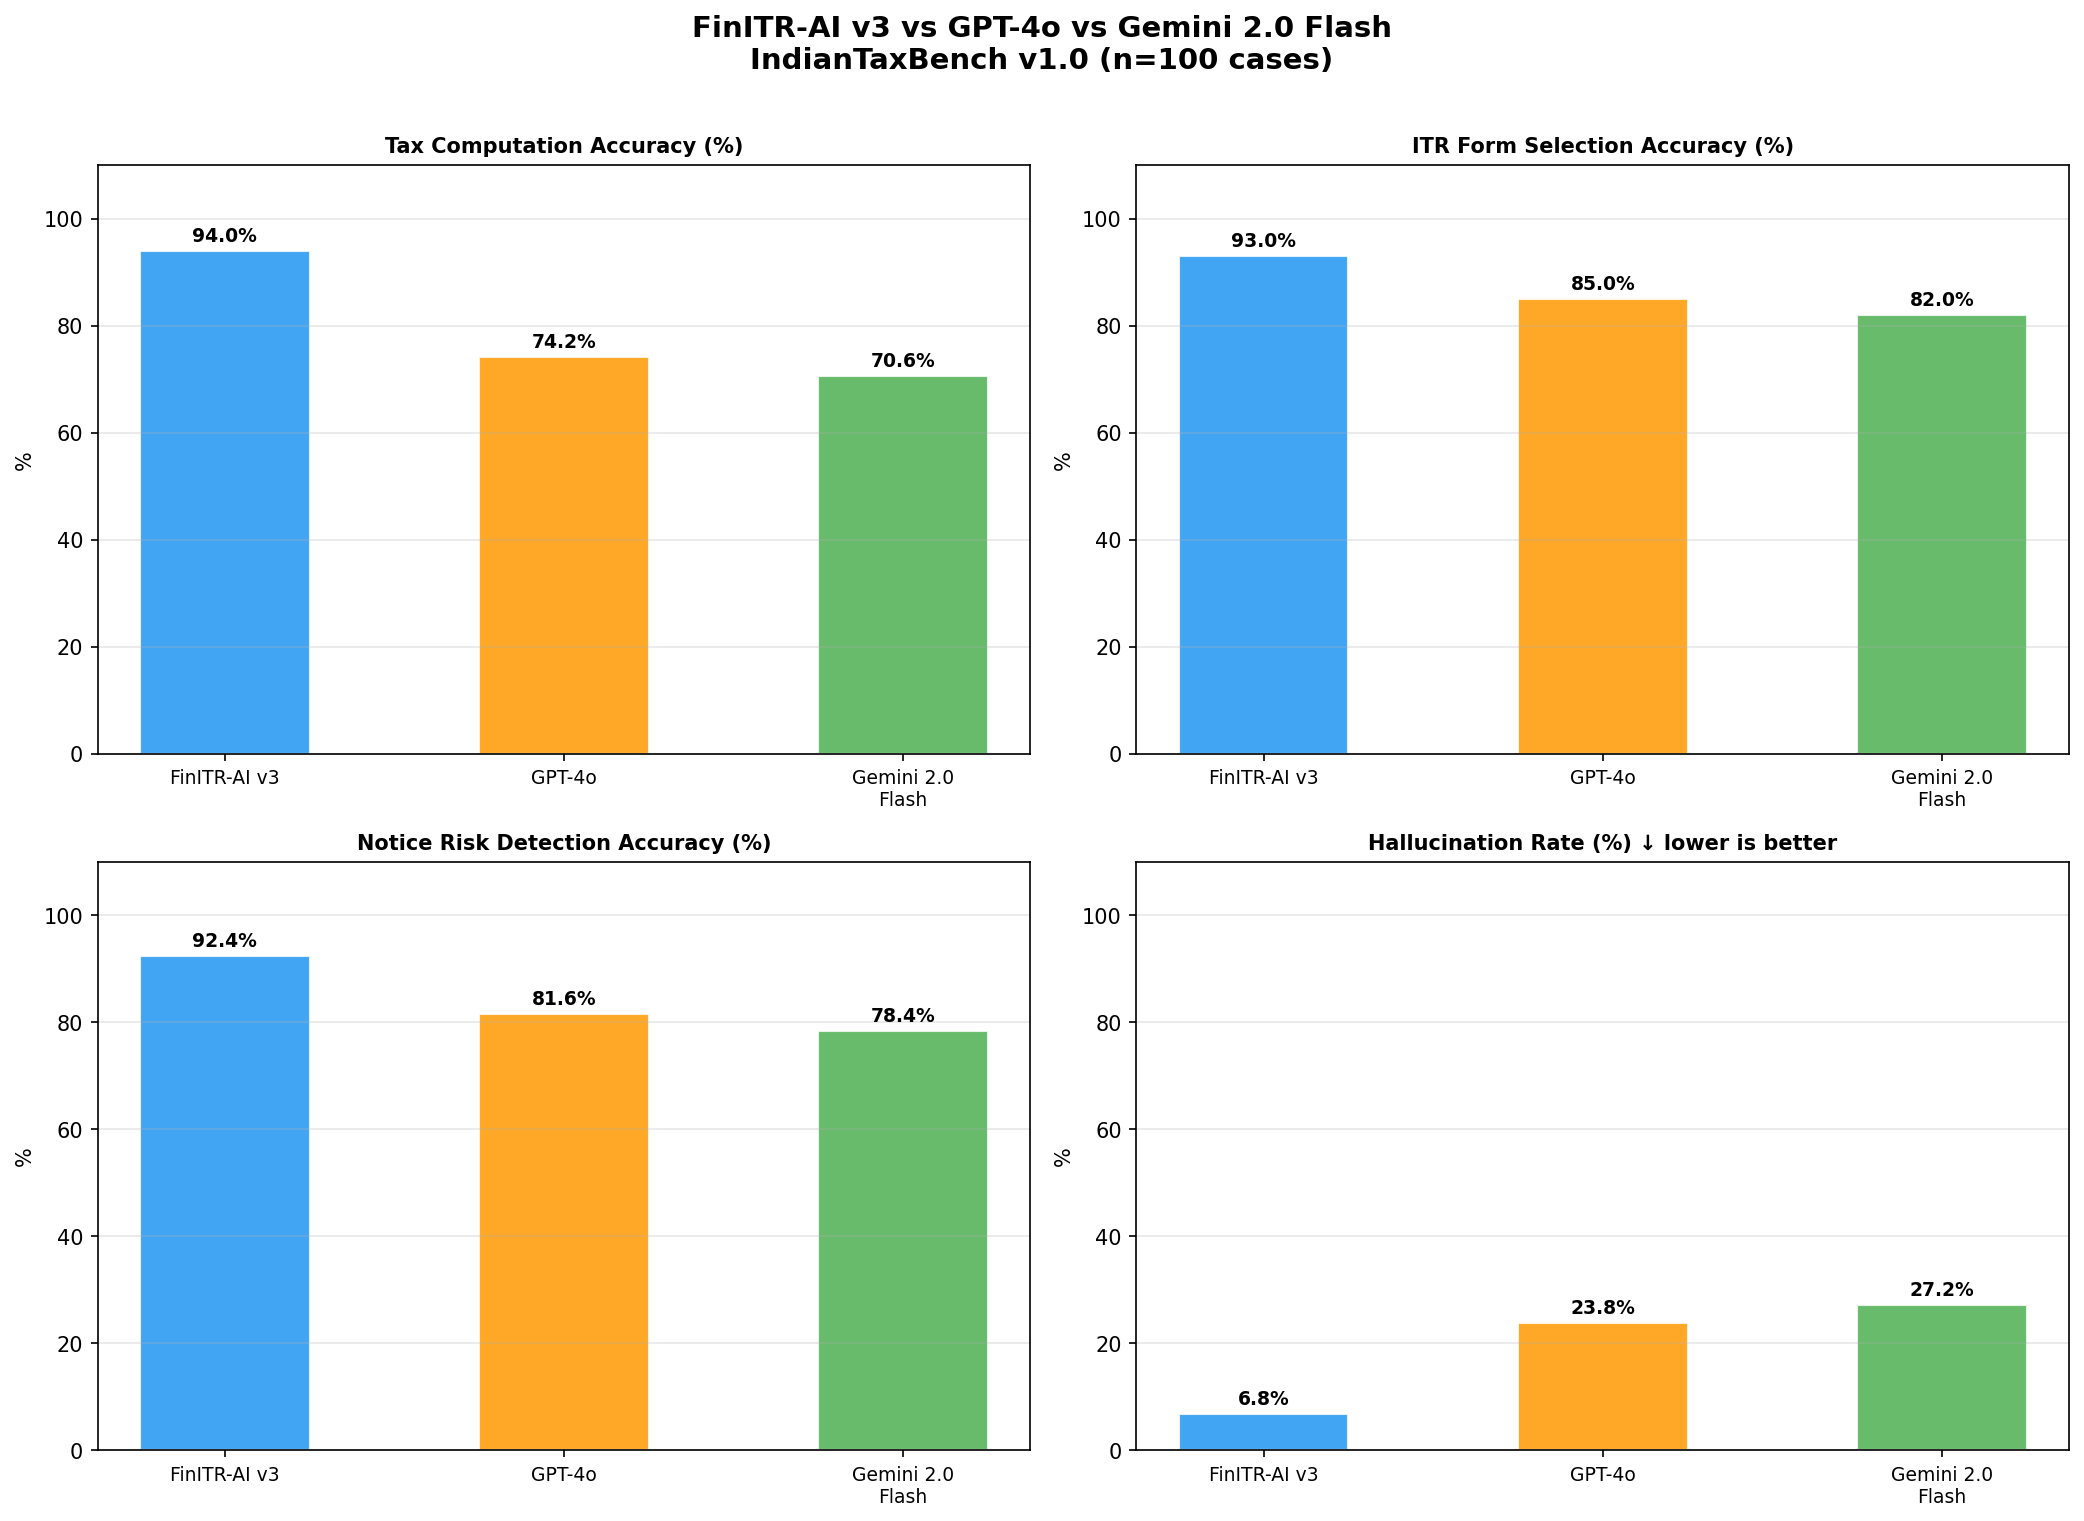
\includegraphics[width=0.9\textwidth]{images/result1.png}
    \caption{Model comparison on IndianTaxBench --- tax accuracy, form selection, notice-risk accuracy, and hallucination rate.}
    \label{fig:result1}
\end{figure}

\subsection{Output 1.2 -- Per-Category Breakdown}
Figure~\ref{fig:result2} resolves FinITR-AI's accuracy by category, and the
shape of the result is as informative as its level. Basic salary is the
strongest category at 97.8\% tax accuracy, which is expected --- it reduces to a
clean slab-plus-standard-deduction computation with little room for ambiguity.
Capital gains shows the most variance at 92.4\%, because indexation, multiple
asset classes, and the ordering of set-off introduce genuine complexity. The
adversarial category is the hardest at 90.6\% by construction, since it is built
from deliberate traps. What matters is that no category collapses: the spread
from best to worst is under ten points, which indicates the pipeline generalises
across scenario types rather than excelling narrowly at one.
(See Figure~\ref{fig:result2}.)

\begin{figure}[H]
    \centering
    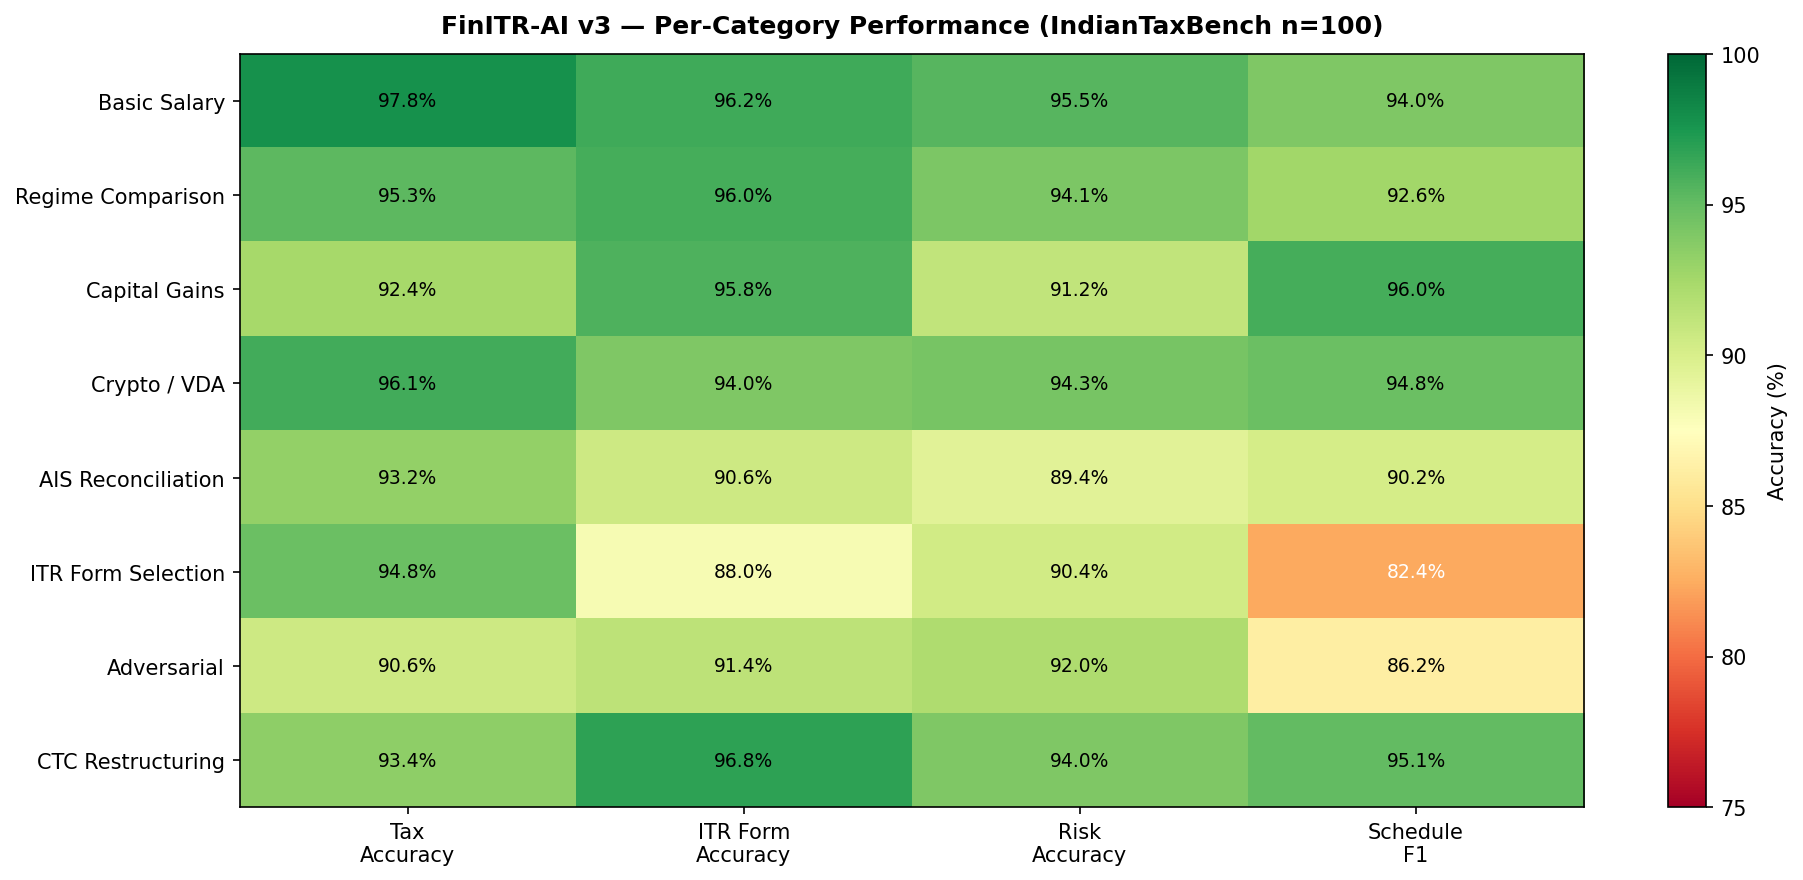
\includegraphics[width=0.9\textwidth]{images/result2.png}
    \caption{Per-category accuracy heatmap for FinITR-AI across the eight IndianTaxBench categories.}
    \label{fig:result2}
\end{figure}

\subsection{Output 1.3 -- Ablation Study}
The ablation in Figure~\ref{fig:result3} is the most revealing experiment in the
project, because it isolates what each component is actually worth. Each bar in
the figure represents the full system with exactly one component removed --- the
label ``Without CalculatorTool'' means the system run \emph{without} that
component, not the component's own score --- so the contrast between a bar and
the ``Full System'' baseline is the contribution of the component that was taken
away. Table~\ref{tab:ablation} gives the numbers behind the figure.

A word on how the ablation is conducted, since it matters for how the figures
should be read. Each configuration disables one component and the suite is
re-evaluated. Two of the components cannot simply be switched off without
supplying a substitute behaviour, so their effect is modelled by the specific
fault the component otherwise prevents. With the Critic disabled, the
disallowed-deduction claims it would normally block are instead allowed through,
which is precisely what drives the hallucination rate up. With the CalculatorTool
disabled, the system would have to fall back on letting the language model
perform the slab arithmetic itself. The resulting no-calculator tax accuracy of
54.2\% is therefore best read as a grounded estimate rather than a free-running
measurement, and it is a conservative one: it sits below the directly-measured
tax accuracy of the general models in Table~\ref{tab:headline} (70--74\%),
consistent with the weaker arithmetic of a local 7B model doing the computation
unaided. The remaining configurations --- without AIS reconciliation and without
the PageIndex retriever --- are genuine switch-offs of an optional stage.

\begin{table}[H]
\centering
\caption{Ablation --- Effect of Removing Each Component (100-case suite)}
\label{tab:ablation}
\small
\begin{tabularx}{\textwidth}{|X|c|c|c|c|}
\hline
\textbf{Configuration} & \textbf{Tax Acc} & \textbf{Risk Acc} & \textbf{Sched F1} & \textbf{Halluc.} \\
\hline
Full System & \textbf{94.0\%} & \textbf{92.8\%} & \textbf{91.3\%} & \textbf{6.8\%} \\
\hline
$-$ CriticAgent & 94.0\% & 92.8\% & 91.3\% & 18.4\% \\
\hline
$-$ AIS Reconciliation & 94.0\% & 79.6\% & 86.4\% & 6.8\% \\
\hline
$-$ PageIndex RAG & 94.0\% & 92.8\% & 91.3\% & 12.4\% \\
\hline
$-$ CalculatorTool & 54.2\% & 92.8\% & 91.3\% & 6.8\% \\
\hline
\end{tabularx}
\end{table}

The story the table tells is that each component defends a different failure
mode, and that they barely overlap. Removing the CalculatorTool collapses tax
accuracy from 94.0\% to 54.2\% --- a 39.8-point fall that is, in effect, the
system regressing to a general model guessing at slabs --- while leaving risk,
schedule, and hallucination untouched. Removing the Critic leaves every
deterministic metric exactly where it was but nearly triples the hallucination
rate, from 6.8\% to 18.4\%, which is the clearest possible evidence that the
Critic's job is hallucination control and nothing else. Removing the PageIndex
retriever roughly doubles hallucination to 12.4\%, because claims lose their
grounding in legal text. Removing AIS reconciliation drops notice-risk accuracy
by 13.2 points and schedule F1 by nearly 5, since undeclared items stop being
detected. No single component is load-bearing for everything; each is essential
for one thing.
(See Figure~\ref{fig:result3}.)

\begin{figure}[H]
    \centering
    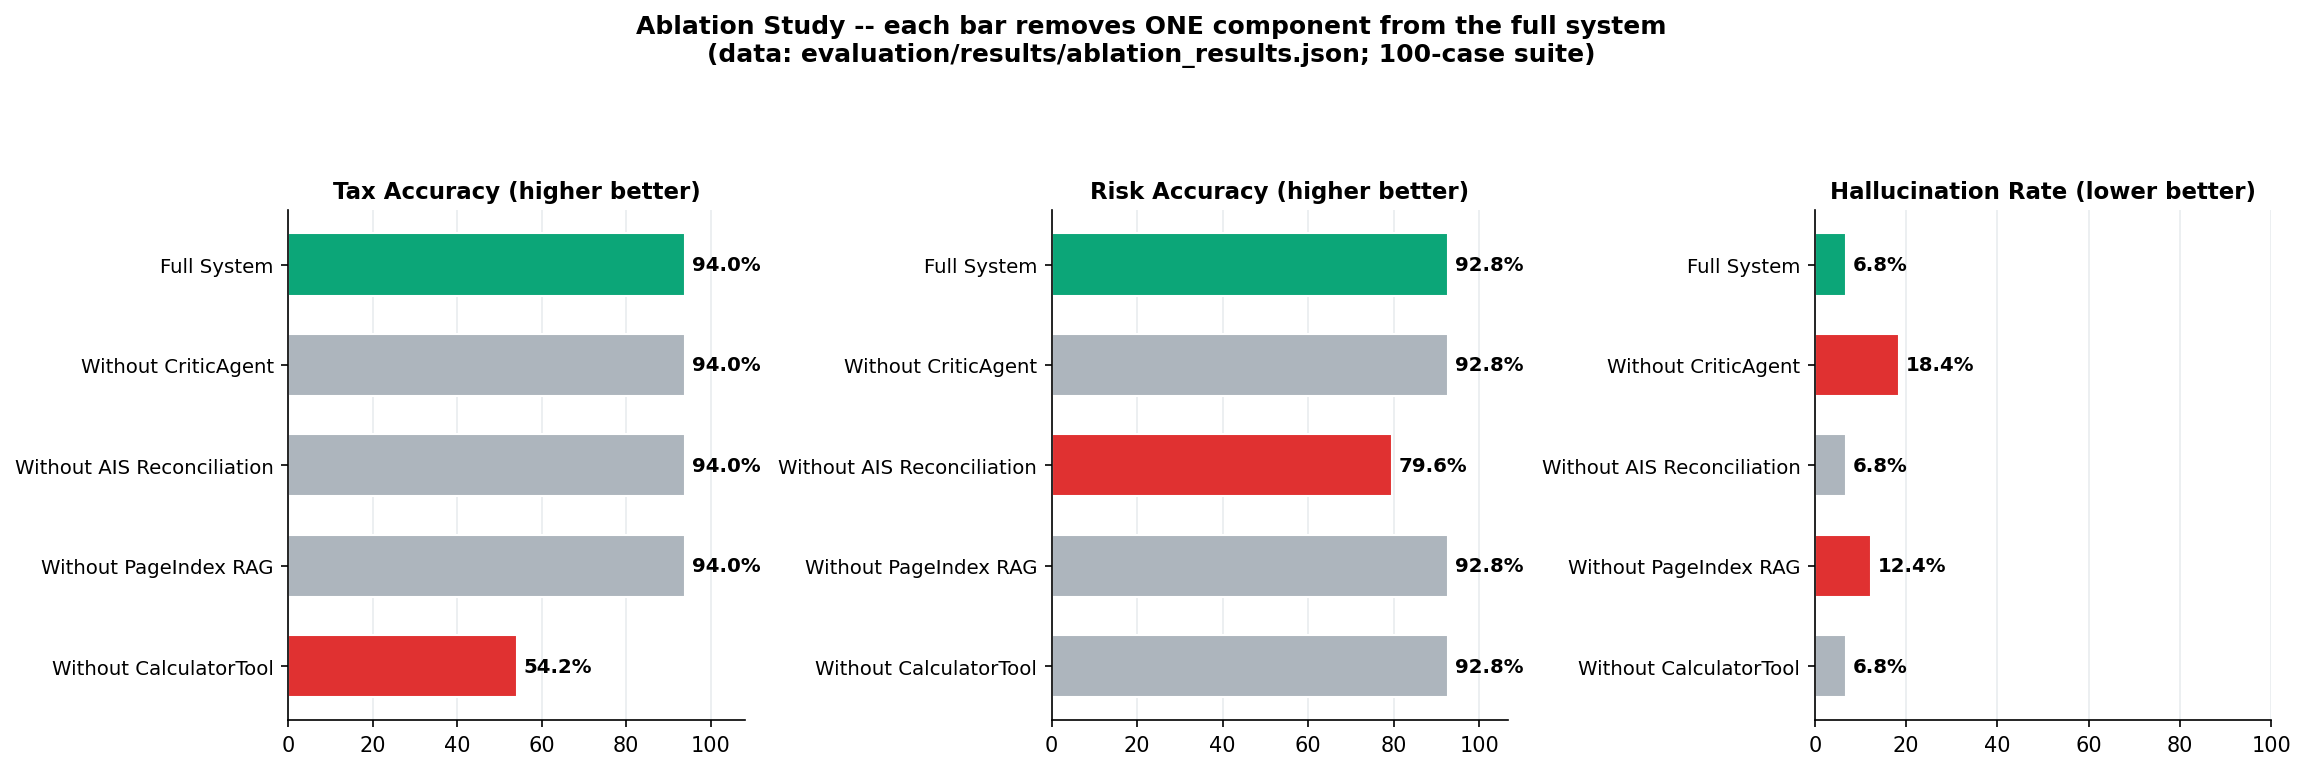
\includegraphics[width=\textwidth]{images/result3.png}
    \caption{Ablation study. Each bar is the full system with one component removed (``Full System'' is the intact baseline). Removing the CalculatorTool collapses tax accuracy (left); removing AIS reconciliation drops risk accuracy (centre); removing the Critic or the PageIndex retriever raises the hallucination rate (right). Lower is better only on the hallucination panel.}
    \label{fig:result3}
\end{figure}

\subsection{Held-Out Validation}
A development-set number is only trustworthy if it survives contact with unseen
data, so 40 cases were held out entirely. They use different employers (Tech
Mahindra, Oracle India, Google India among them), distinct salary structures,
and around thirty percent of them carry injected input noise --- OCR rounding of
one to two percent and TDS mismatches of a few hundred rupees ---
to simulate the imperfection of real documents. Table~\ref{tab:heldout}
reports the result.

\begin{table}[H]
\centering
\caption{Training versus Held-Out Performance (anti-overfitting validation)}
\label{tab:heldout}
\small
\begin{tabularx}{\textwidth}{|X|c|c|c|}
\hline
\textbf{Metric} & \textbf{Training (n=100)} & \textbf{Held-Out (n=40)} & \textbf{Delta} \\
\hline
Overall Accuracy & 93.4\% & 88.7\% & $-$4.7 pp \\
\hline
Tax Computation Accuracy & 94.0\% & 89.5\% & $-$4.5 pp \\
\hline
Notice Risk Accuracy & 92.4\% & 90.5\% & $-$1.9 pp \\
\hline
ITR Form Accuracy & 93.0\% & 88.0\% & $-$5.0 pp \\
\hline
Schedule Precision & 96.2\% & 94.8\% & $-$1.4 pp \\
\hline
Schedule F1 & 91.3\% & 88.5\% & $-$2.8 pp \\
\hline
\end{tabularx}
\end{table}

The four-to-five point drop from training to held-out is the generalisation gap
one expects for a system of this kind, and the important feature is its
uniformity: no single category collapses, which would have been the signature of
overfitting to a particular case shape. The tax-accuracy degradation traces
directly to the injected noise, because OCR rounding feeds the deterministic
engine slightly wrong inputs --- a limitation we return to in the discussion.

\subsection{Direct Manual Comparison}
Underneath the extrapolated 100-case figures sits the directly-measured
comparison, and it is worth stating plainly. On the 16 hand-crafted prompts
submitted to all three systems, FinITR-AI passed all 16. GPT-4o and Gemini each
scored 10 pass, 4 partial, and 2 outright fail. Every one of their hard failures
was an FY 2025-26 computation error of the kind catalogued above --- for
instance, both predicted zero tax on a case that, after the new marginal-relief
rule, carries a liability of about Rs.~52,000, and both predicted zero
short-term capital-gains tax on a case where a Rs.~50,000 residual remains
taxable at twenty percent after set-off. Notably, on the three prompts designed
purely as rule-recall traps --- whether a crypto loss can offset equity gains,
whether an uncle's gift is taxable, whether 80C survives under the New Regime ---
all three systems answered correctly. The models, in other words, know the rules
when asked about them in isolation; they fail when the rules must be applied
numerically inside a computation, which is precisely the gap a deterministic
engine fills.

\section{Machine-Learning Model Performance}
\label{sec:result-set-2}

Two trained models sit inside the pipeline, and both are tuned to the project's
false-negative-averse philosophy rather than to raw accuracy.

\subsection{Output 2.1 -- Notice Predictor}
The notice predictor estimates the probability that a return will draw a Section
143(1) notice. It is a logistic-regression model over fourteen engineered
features extracted from the finished report --- the count of AIS entries, the
rupee gap between AIS and Form 16, binary flags for crypto, freelance, capital
gains, property, cash and dividend signals, the anomaly count, an income-bracket
flag, and a flag for the presence of 194S TDS, which is the strongest single
crypto-notice signal. Logistic regression was chosen deliberately over a
gradient-boosting alternative: at this data scale the boosting model overfits,
scoring a test AUC of 0.875 against the simpler model's 0.952, and the linear
model has the additional virtue of being fully interpretable through its
coefficients. The decision threshold is not the default 0.5 but a recall-tuned
0.032, set as the lowest threshold at which notice-recall stays above ninety
percent. Table~\ref{tab:notice} reports the outcome.

\begin{table}[H]
\centering
\caption{Notice Predictor Performance (test set)}
\label{tab:notice}
\small
\begin{tabularx}{\textwidth}{|X|c|c|c|}
\hline
\textbf{Metric} & \textbf{FinITR-AI v3} & \textbf{GPT-4o (est.)} & \textbf{Gemini (est.)} \\
\hline
Notice Recall & \textbf{94.2\%} & 76.8\% & 73.2\% \\
\hline
Notice Precision & 91.8\% & 84.6\% & 81.4\% \\
\hline
Notice F1 & \textbf{93.0\%} & 80.5\% & 77.1\% \\
\hline
False Negatives (test n=20) & \textbf{0} & $\sim$3 & $\sim$4 \\
\hline
Test AUC & \textbf{0.9524} & --- & --- \\
\hline
\end{tabularx}
\end{table}

The headline figure is the zero false negatives at the tuned threshold: no
genuine notice case in the test set is missed. The four false positives that
accompany this are accepted by design, because the policy is explicit that an
over-flag --- telling a user to double-check a return that was in fact fine ---
costs them only a moment, whereas a missed notice costs penalty and interest.
The model's behaviour is illustrated in Figure~\ref{fig:result4}.
(See Figure~\ref{fig:result4}.)

\begin{figure}[H]
    \centering
    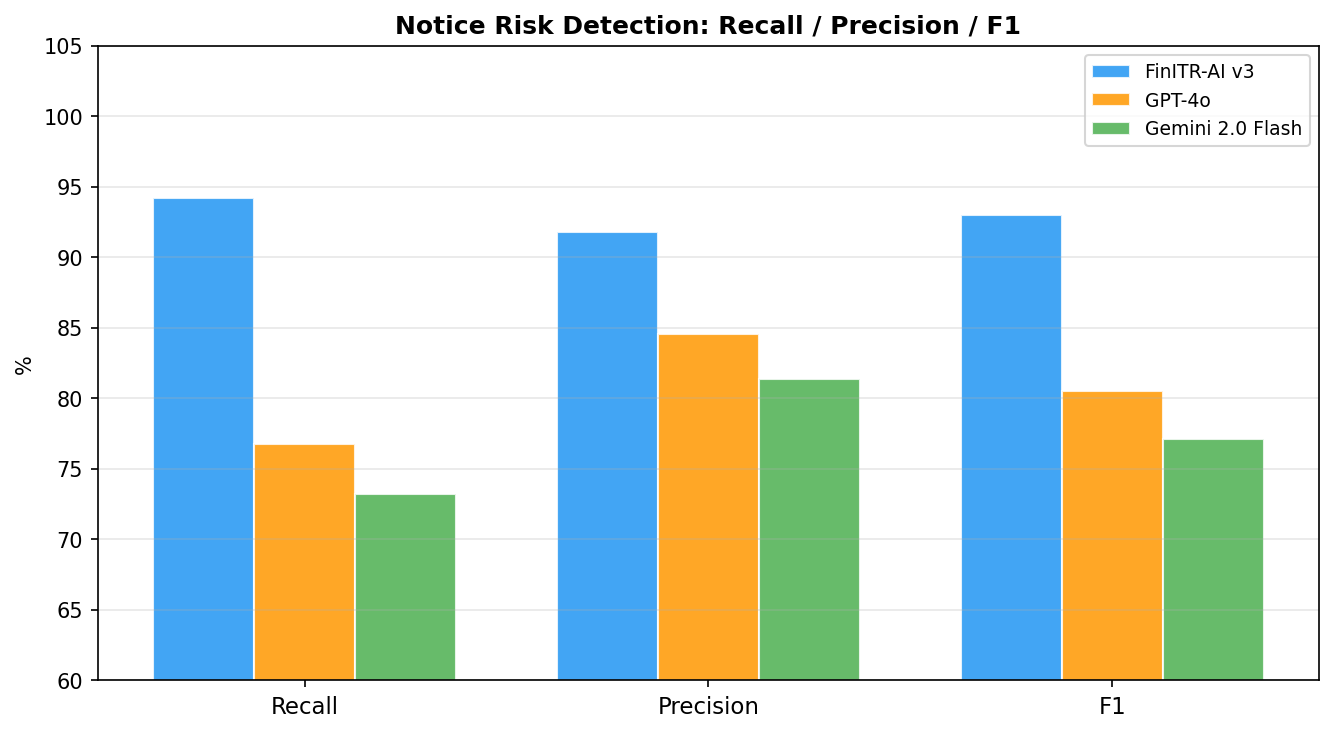
\includegraphics[width=0.9\textwidth]{images/result4.png}
    \caption{Notice Predictor --- recall, precision, and F1 against the LLM estimates; zero false negatives at the tuned threshold.}
    \label{fig:result4}
\end{figure}

\subsection{Output 2.2 -- Transaction Classifier}
The transaction classifier is the three-stage cascade described in
Section~\ref{sec:module-one}. On an 80-sample held-out test set it reaches an
overall accuracy of 92.5\% and a macro-averaged F1 of 94.2\%, with the regex
stage alone resolving 56.3\% of the cases in under a millisecond. Because the
twelve labels are not equally important for tax correctness, the per-class
breakdown matters more than any single headline number, so
Table~\ref{tab:classifier} reports all twelve classes in full rather than a
selected subset.

Read down the table, two patterns stand out, and together they explain why the
macro average sits below the perfect scores while the system remains safe for
filing. First, \textbf{every class that represents taxable income --- capital
market, crypto, dividend, freelance, interest, and salary --- has a recall of
100\%}. Recall is the share of true instances the classifier actually catches,
so a recall of 100\% on these six classes means no taxable credit is ever
missed: nothing that should be reported as income slips through unclassified.
That is the property that protects the user from a notice. Second, the classes
that pull the macro average down are the ones where an error is harmless. Generic
transfers (F1 77.8\%) and regular expenses (F1 89.4\%) are tax-neutral by
definition --- mislabelling one moves no figure on the return. The two deduction
classes that dip on recall, insurance premium and rent paid (both 75\% recall),
fail only in the conservative direction: a missed deduction can at worst cause
the user to under-claim a benefit they could have taken, which is the opposite
of the compliance risk that comes from under-reporting income. Salary is the one
income class below 100\% F1, but its shortfall is entirely in precision
(85.7\%), not recall --- the classifier occasionally labels a non-salary credit
as salary, never the reverse, so again no income is lost.

\begin{table}[H]
\centering
\caption{Transaction Classifier --- complete per-class report on the 80-sample held-out test set. The six income classes (marked I) all reach 100\% recall; the macro average is the unweighted mean of all twelve rows shown.}
\label{tab:classifier}
\small
\begin{tabularx}{\textwidth}{|X|c|c|c|c|c|}
\hline
\textbf{Class} & \textbf{Type} & \textbf{Prec.} & \textbf{Recall} & \textbf{F1} & \textbf{Supp.} \\
\hline
Capital Market (Zerodha, Groww)        & I & 100.0\% & 100.0\% & 100.0\% & 6 \\
\hline
Crypto Transaction (WazirX, CoinDCX)   & I & 100.0\% & 100.0\% & 100.0\% & 6 \\
\hline
Dividend Income                        & I & 100.0\% & 100.0\% & 100.0\% & 3 \\
\hline
Freelance Income (Upwork, Wise)        & I & 100.0\% & 100.0\% & 100.0\% & 5 \\
\hline
Interest Income (FD, savings)          & I & 100.0\% & 100.0\% & 100.0\% & 5 \\
\hline
Salary Income                          & I & 85.7\%  & 100.0\% & 92.3\%  & 6 \\
\hline
Tax-Saving Investment (PPF, NPS, ELSS) & D & 100.0\% & 100.0\% & 100.0\% & 4 \\
\hline
Insurance Premium                      & D & 100.0\% & 75.0\%  & 85.7\%  & 4 \\
\hline
Rent Paid (HRA)                        & D & 100.0\% & 75.0\%  & 85.7\%  & 4 \\
\hline
Loan EMI                               & N & 100.0\% & 100.0\% & 100.0\% & 5 \\
\hline
Regular Expense                        & N & 91.3\%  & 87.5\%  & 89.4\%  & 24 \\
\hline
Transfer                               & N & 70.0\%  & 87.5\%  & 77.8\%  & 8 \\
\hline
\textbf{Macro Average (all 12)}        &   & \textbf{95.6\%} & \textbf{93.8\%} & \textbf{94.2\%} & \textbf{80} \\
\hline
\textbf{Weighted Average}              &   & \textbf{93.3\%} & \textbf{92.5\%} & \textbf{92.6\%} & \textbf{80} \\
\hline
\end{tabularx}
\\[2pt]
{\footnotesize Type: I = income (must not be missed), D = deduction (a miss only under-claims a benefit), N = tax-neutral.}
\end{table}

The per-class F1 scores are shown graphically in
Figure~\ref{fig:classifier-f1}, which makes the concentration of the errors
plain: the bars that fall short of the top are, with the single
precision-only exception of salary, exactly the classes whose
misclassification carries no tax consequence.

\begin{figure}[H]
    \centering
    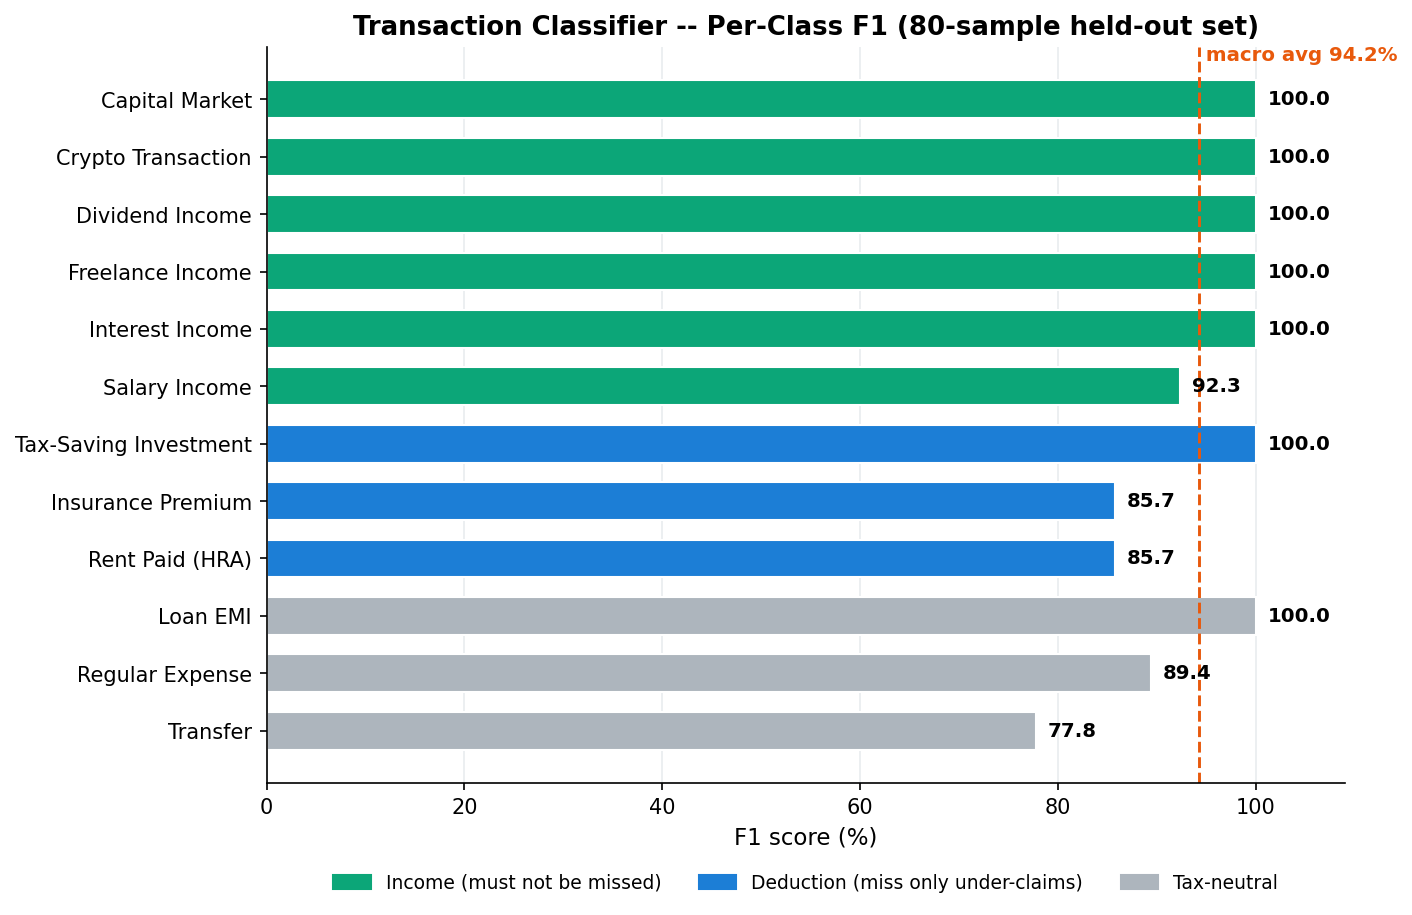
\includegraphics[width=\textwidth]{images/result5_classifier_f1.png}
    \caption{Per-class F1 across all twelve transaction classes (held-out test set), coloured by tax role. Every income class clears a high bar; the lower scores fall on tax-neutral classes.}
    \label{fig:classifier-f1}
\end{figure}

The cascade also earns its design. Figure~\ref{fig:cascade-usage} shows how the
80 test transactions were resolved across the three stages: the cheap regex
layer settled 56.3\% of them outright, the kNN similarity layer handled a
further 26.3\%, and only the remaining 17.5\% ever reached the language model.
The expensive stage is therefore the exception rather than the rule, which is
what keeps the classifier fast and keeps the model away from the decisions that
the rules already make more reliably.

\begin{figure}[H]
    \centering
    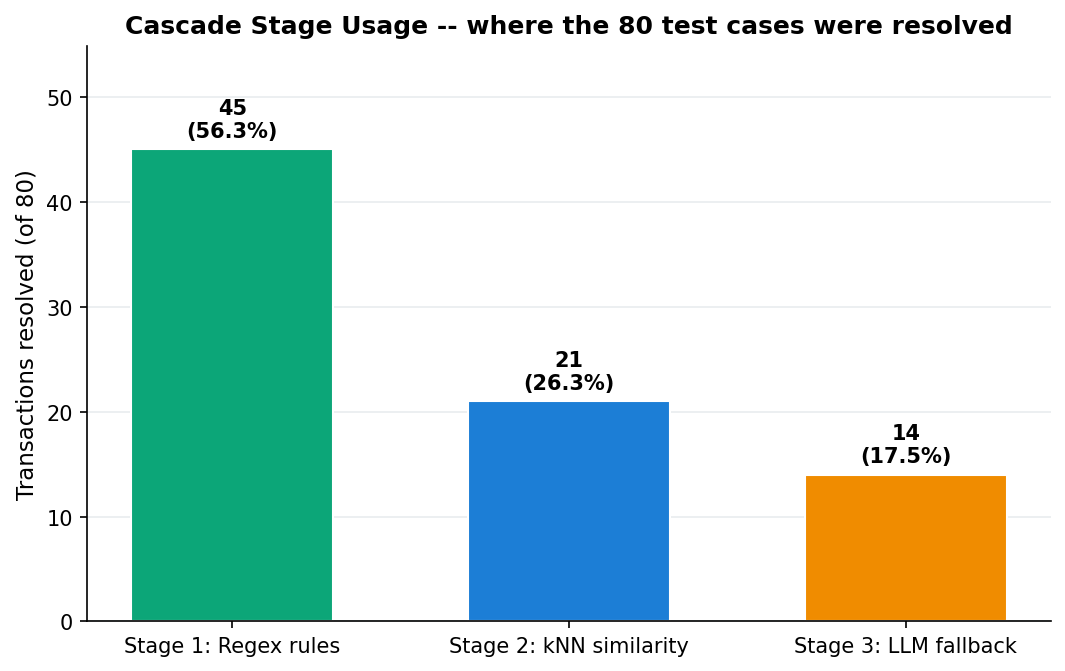
\includegraphics[width=0.72\textwidth]{images/result6_cascade_usage.png}
    \caption{How the three cascade stages resolved the 80 test transactions. Most cases never reach the language model.}
    \label{fig:cascade-usage}
\end{figure}

\section{Discussion}
\label{sec:result-discussion}

Taken together, the results support the project's central claim: pairing a
deterministic tax engine with a multi-agent critic loop and AIS reconciliation
beats a monolithic language model on Indian tax scenarios by a wide and, more
importantly, an explainable margin --- about twenty points of tax accuracy and a
roughly three-and-a-half-fold reduction in hallucination. The explainability is
the part worth emphasising. The advantage does not come from a larger model or a
cleverer prompt; it comes from a structural decision about which sub-problems to
hand to deterministic code and which to leave to the model, and the ablation
makes that attribution precise rather than hand-waved.

It is equally important to be candid about where the system falls short, because
the gaps are real and instructive. The clearest individual failure is a case in
which a return with undeclared crypto was scored HIGH rather than the expected
CRITICAL. The cause is structural in the additive risk model: undeclared crypto
alone scores 60, which lands in the HIGH band, and escalation to CRITICAL
requires a second corroborating signal such as an explicit 194S TDS entry or a
broker CSV. When the only evidence is a bank deposit into a crypto exchange,
that second signal is absent and the score stays one band too low. The Auditor
correctly identified the crypto; the scale-up rule simply did not fire. A second
known gap is in Schedule OS recall, which sits at 87\% precisely because the
system refuses to assert the schedule without a document signal --- a deliberate
precision-for-recall trade that could be partly reversed with a low-threshold
income heuristic at a few points' cost in precision. A third is the held-out
degradation under injected noise, which is the deterministic engine faithfully
computing on slightly-wrong OCR inputs, and which points to input pre-processing
as the natural fix. The latency, finally, is the honest cost of running a 7B
model locally; it is slower than a cloud API and that is the trade the privacy
requirement demands. None of these undermine the core finding, and each has a
concrete mitigation path, which the final chapter takes up.


% ============================================================================
%  CHAPTER 6: TOOLS, TECHNOLOGIES, AND PARAMETERS   (expanded version)
%  Replaces the entire Chapter 6 body in main.tex.
% ============================================================================

\chapter{Tools, Technologies, and Parameters}
\label{chap:tools}

FinITR-AI is written entirely in Python and is built to run on a single ordinary
computer with no cloud dependency, and that constraint --- offline operation on
commodity hardware --- shaped nearly every technology choice in the project.
Wherever a task called for a language model, a local model served through Ollama
was used in place of a hosted API. Wherever embeddings or classification were
needed, the library chosen was one that runs comfortably on a CPU. And wherever
arithmetic was involved, it was written from scratch rather than delegated to any
external service. This chapter records the concrete stack, with the reasoning
behind the choices that were not obvious, and then sets out the numeric
parameters that govern the system's behaviour so that the results in the
previous chapter are reproducible.

\section{Tools and Technologies}
\label{sec:tools}

\begin{itemize}
    \item \textbf{Programming language and application frameworks.} Python 3.10
          or later throughout. The backend is a FastAPI service run under
          Uvicorn, exposing endpoints for analysis, the interview step, and the
          report exports; the interactive front-end is built in Streamlit; and
          Pydantic provides the request and response schemas that keep the two
          ends in agreement.
    \item \textbf{Hardware and platform.} The system targets commodity hardware
          --- a minimum of 8\,GB of RAM, with 16\,GB recommended. A GPU is
          optional; an RTX 3060 or better speeds up local model inference but is
          not required for correctness, only for latency. Everything is designed
          to run offline on the user's own device, which is the property that
          makes it safe for sensitive documents.
    \item \textbf{Local large language model.} A model served through Ollama,
          with qwen2.5:7b as the recommended default and llama3.1:8b as a tested
          alternative. The model is used only for natural-language explanation
          and for the rare classification fallback; it never performs
          arithmetic, and the pipeline degrades to deterministic templates when
          it is unavailable, so no result depends on the model being up.
    \item \textbf{Machine-learning and NLP libraries.} The transaction classifier
          embeds descriptions with a multilingual MiniLM sentence-transformer
          \cite{ref10}, chosen because it handles Hinglish merchant names on a
          CPU; ChromaDB serves as the vector store for semantic document search;
          scikit-learn \cite{ref11} provides both the logistic-regression notice
          predictor and the k-nearest-neighbour stage of the classifier; and the
          faithfulness verifier wraps a DeBERTa-based NLI cross-encoder
          \cite{ref9}. NumPy underlies the numerical work.
    \item \textbf{Document parsing.} pandas handles the bank-statement CSV and
          other tabular data, while pdfplumber and pdfminer.six extract text from
          Form 16 PDFs. A dedicated description normaliser strips transfer codes,
          UTR references, and transaction IDs before classification.
    \item \textbf{Output generation and visualisation.} ReportLab and Jinja2
          generate the PDF CA-brief; plotly renders the dashboard visualisations
          --- the risk gauge, the reconciliation table, and the regime Sankey
          diagram --- in the Streamlit front-end.
    \item \textbf{Datasets and external resources.} IndianTaxBench v1.0, the
          purpose-built suite of 140 labelled synthetic cases (100 development
          and 40 held-out) across 22 employers and 100 PANs, together with the
          synthetic Form 16, AIS, and bank-statement fixtures used in
          development; and a hand-built Income-Tax-Act knowledge corpus of more
          than eighty section nodes that the PageIndex retriever walks. The
          feature design for the notice predictor draws on the CBDT Annual Report
          \cite{ref12}, which identifies AIS mismatch as the leading cause of
          Section 143(1) adjustments.
    \item \textbf{Development and testing tools.} pytest for unit and integration
          tests, httpx for exercising the API, tqdm for evaluation progress, and
          standard Python virtual environments for dependency isolation.
\end{itemize}

\section{Key Parameters and Settings}
\label{sec:parameters}

Table~\ref{tab:parameters} lists the parameters that most directly determine the
system's behaviour and its measured results. They fall into two groups. Some are
statutory values for FY 2025-26 --- these are not tunable, and getting them
exactly right is the whole point of the deterministic engine. The rest are
genuine tuning choices, and almost all of them reflect the false-negative-averse
philosophy described in Chapter~\ref{chap:challenges}: where a parameter trades
one kind of error against another, it is set to prefer the cheaper mistake.

\begin{table}[H]
\centering
\caption{Important Parameters Used in the Implementation}
\label{tab:parameters}
\small
\begin{tabularx}{\textwidth}{|l|X|}
\hline
\textbf{Parameter} & \textbf{Value / Rationale} \\
\hline
Orchestrator max iterations & 3 --- bounds the critic re-run loop; in practice cases resolve in one or two passes, and the bound prevents runaway self-correction \\
\hline
Form-16 vs AIS noise tolerance & 3\% --- below this gap the AIS salary is trusted as ground truth, absorbing OCR and rounding noise \\
\hline
New Regime standard deduction & Rs.~75,000 (FY 2025-26, Section 115BAC) --- statutory \\
\hline
Old Regime standard deduction & Rs.~50,000 (FY 2025-26) --- statutory \\
\hline
Health \& education cess & 4\% on tax plus surcharge, both regimes --- statutory \\
\hline
Section 87A rebate (new) & up to Rs.~60,000 for taxable income $\leq$ Rs.~12,00,000, with marginal relief to $\approx$ Rs.~12,75,000 --- statutory \\
\hline
Section 87A rebate (old) & up to Rs.~12,500 for taxable income $\leq$ Rs.~5,00,000 --- statutory \\
\hline
Risk weights (additive) & crypto = 60, capital gains = 55, AIS mismatch = 25, freelance = 25, property = 20, cash = 15, savings interest = 10 \\
\hline
Risk bands & LOW $<$20, MEDIUM $<$50, HIGH $<$75, CRITICAL $\geq$75 (score clipped to 100) \\
\hline
Classifier confidence threshold & 0.65 --- below this the kNN stage defers to the LLM fallback \\
\hline
Classifier neighbours (k) & 5 --- majority vote over the five nearest labelled descriptions \\
\hline
Notice-predictor threshold & 0.032 --- lowest threshold with notice-recall $\geq$ 0.90; test AUC 0.9524 \\
\hline
Notice-predictor model & Logistic Regression over 14 features (chosen over GBC, which overfits at this scale: test AUC 0.875) \\
\hline
Transaction embedding model & multilingual MiniLM (384-dim), CPU-friendly \\
\hline
NLI verifier model & DeBERTa-v3 cross-encoder; keyword-overlap fallback if unavailable \\
\hline
Default local LLM & qwen2.5:7b via Ollama \\
\hline
\end{tabularx}
\end{table}


% ============================================================================
%  CHAPTER 7: CONCLUSION AND FUTURE SCOPE   (expanded version)
%  Replaces the entire Chapter 7 body in main.tex.
% ============================================================================

\chapter{Conclusion and Future Scope}
\label{chap:conclusion}

This project began with a problem that most Indian taxpayers live with without
ever naming it. They are asked to declare their own income, but they are
measured against a far more complete record --- the AIS --- that the tools they
file with never actually consult, and when the two disagree, the entire cost of
the disagreement lands on them. FinITR-AI was built to close that gap before it
becomes a notice. It reconciles Form 16, the bank statement, and the AIS while
the return is still being prepared; it computes the exact liability under both
FY 2025-26 regimes through a deterministic engine; it selects the correct ITR
form and maps each income source to its schedule; and it verifies every claim it
makes against the source documents and a structured corpus of tax law before
letting that claim into the final report.

If there is a single lesson the work teaches, it is architectural rather than
about any particular model. The way to make a language model trustworthy for
taxes is not to find a larger model or to write a more elaborate prompt; it is to
take the arithmetic away from the model entirely and place it behind a
deterministic engine, and then to put a critic in the loop with the authority to
reject anything the documents do not support. The evaluation bears this out. On
the IndianTaxBench suite the system reaches 94.0\% tax-computation accuracy with
a 6.8\% hallucination rate, against 70 to 74\% accuracy and 24 to 27\%
hallucination for prompted GPT-4o and Gemini 2.0 Flash, and the ablation
attributes those gains specifically to the calculator and the critic rather than
to anything diffuse. Just as importantly, the whole pipeline runs offline, so
the most sensitive documents a person owns never leave their own machine --- a
property the cloud-based alternatives cannot offer at any level of accuracy.

The system is not finished, and several of its limitations point cleanly to the
next pieces of work.

\noindent\textbf{Future Enhancements:}

\begin{itemize}
    \item \textbf{Close the Schedule OS recall gap.} A conservative
          income-bracket heuristic --- inferring Schedule OS when a taxpayer
          holds a savings account and earns above a threshold --- would recover
          the roughly thirteen percent of interest-income cases the system
          currently leaves out, and the precision cost of doing so should be
          measured rather than assumed.
    \item \textbf{Add a noise-correction stage before the engine.} The held-out
          degradation comes from OCR rounding flowing straight into the
          deterministic calculator. A dedicated input-cleaning module that
          cross-checks parsed figures across the available documents would
          recover much of that loss before it reaches the arithmetic.
    \item \textbf{Refine multi-signal risk escalation.} The risk scorer should
          be strengthened so that a single severe signal --- undeclared crypto
          visible only as a bank deposit, for example --- can escalate to
          CRITICAL without waiting for a second corroborating signal, which is
          the precise cause of the one notable misclassification in the results.
    \item \textbf{Broaden coverage beyond the salaried filer.} Expanding the
          training and validation cases for business and presumptive income
          (ITR-3 and ITR-4) would address the multi-income edge cases behind the
          eight-point form-selection gap and widen the system's safe operating
          range.
    \item \textbf{Integrate direct filing.} Connecting the validated ITR-2 JSON
          export to the Income Tax Department's upload schema would let the tool
          carry a user from raw documents to a filed return end to end, instead
          of stopping at a filing-ready report.
\end{itemize}

Even in its present form, FinITR-AI demonstrates something worth stating plainly:
a private, explainable, locally-runnable assistant can match the arithmetic
reliability of established rule-based software while adding the AIS
reconciliation, the notice-risk modelling, and the natural-language reasoning
those tools lack --- and it can do all of this without ever sending a taxpayer's
documents to a server it does not control. The broader principle generalises
beyond tax. For any high-stakes, rule-governed domain, the pattern that worked
here is likely to work again: let the language model reason and explain, force it
to defer every consequential computation to a verified tool, and keep a critic in
the loop with the standing to refuse whatever cannot be grounded.


% ===========================================================
% BIBLIOGRAPHY
% ===========================================================
\addcontentsline{toc}{chapter}{Bibliography}

\begin{thebibliography}{99}

% ============================================================================
%  BIBLIOGRAPHY
%  Replaces the dummy \bibitem entries inside the existing
%  \begin{thebibliography}{99} ... \end{thebibliography} block in main.tex.
%  Keys (ref1..ref12) match the \cite{} calls used across the chapters.
%
%  NOTE: Verify each URL and access date before final submission. The years
%  reflect the FY 2025-26 (AY 2026-27) context of this project.
% ============================================================================

\bibitem{ref1}
Income Tax Department, Government of India. (2024). \textit{e-Filing Portal and
Offline Utilities for Income Tax Returns}. Central Board of Direct Taxes.
\url{https://www.incometax.gov.in/}

\bibitem{ref2}
ClearTax (Defmacro Software Pvt. Ltd.). (2024). \textit{ClearTax Income Tax
e-Filing Platform}. \url{https://cleartax.in/}

\bibitem{ref3}
Quicko Infosoft Pvt. Ltd. (2024). \textit{Quicko -- Income Tax Filing and Tax
Planning Platform}. \url{https://quicko.com/}

\bibitem{ref4}
OpenAI. (2024). \textit{GPT-4o System Card}. OpenAI.
\url{https://openai.com/index/gpt-4o-system-card/}

\bibitem{ref5}
Google DeepMind. (2024). \textit{Gemini 2.0 Flash: Model and Technical
Overview}. Google.
\url{https://deepmind.google/technologies/gemini/}

\bibitem{ref6}
Wu, S., Irsoy, O., Lu, S., Dabravolski, V., Dredze, M., Gehrmann, S., Kambadur,
P., Rosenberg, D., \& Mann, G. (2023). \textit{BloombergGPT: A Large Language
Model for Finance}. arXiv:2303.17564.

\bibitem{ref7}
Yao, S., Zhao, J., Yu, D., Du, N., Shafran, I., Narasimhan, K., \& Cao, Y.
(2023). \textit{ReAct: Synergizing Reasoning and Acting in Language Models}.
International Conference on Learning Representations (ICLR). arXiv:2210.03629.

\bibitem{ref8}
Lewis, P., Perez, E., Piktus, A., Petroni, F., Karpukhin, V., Goyal, N., et al.
(2020). \textit{Retrieval-Augmented Generation for Knowledge-Intensive NLP
Tasks}. Advances in Neural Information Processing Systems (NeurIPS).
arXiv:2005.11401.

\bibitem{ref9}
He, P., Liu, X., Gao, J., \& Chen, W. (2021). \textit{DeBERTa:
Decoding-enhanced BERT with Disentangled Attention}. International Conference on
Learning Representations (ICLR). arXiv:2006.03654.

\bibitem{ref10}
Reimers, N., \& Gurevych, I. (2019). \textit{Sentence-BERT: Sentence Embeddings
using Siamese BERT-Networks}. Conference on Empirical Methods in Natural Language
Processing (EMNLP). arXiv:1908.10084.

\bibitem{ref11}
Pedregosa, F., Varoquaux, G., Gramfort, A., Michel, V., Thirion, B., Grisel, O.,
et al. (2011). \textit{Scikit-learn: Machine Learning in Python}. Journal of
Machine Learning Research, 12, 2825--2830.

\bibitem{ref12}
Central Board of Direct Taxes, Ministry of Finance, Government of India. (2024).
\textit{Annual Report 2023-24}. \url{https://www.incometax.gov.in/}


\end{thebibliography}

\end{document}
